% IEEE Robotics and Automation Letters (RA-L) — Türkçe taslak
% Başlık: ROS 2 Navigasyonu için Belirsizlik-Duyarlı Negatif Engel Risk Temsili

\documentclass[journal]{IEEEtran}

\usepackage[utf8]{inputenc}
\usepackage[T1]{fontenc}
\usepackage{amsmath,amssymb,amsfonts}
\usepackage{algorithmic}
\usepackage{algorithm}
\usepackage{graphicx}
\usepackage{textcomp}
\usepackage{xcolor}
\usepackage{cite}
\usepackage{booktabs}
\usepackage{url}
\usepackage{hyperref}
\usepackage{multirow}
\usepackage{array}

\graphicspath{{figures/}}

\newcommand{\fsr}{\mathrm{YHO}}
\newcommand{\drop}{\textsc{Drop}}
\newcommand{\safe}{\textsc{Guvenli}}
\newcommand{\unc}{\textsc{Belirsiz}}
\newcommand{\solid}{\textsc{Kati}}
\newcommand{\R}{\mathbb{R}}
\newcommand{\Z}{\mathbb{Z}}

\begin{document}

\title{ROS~2 Navigasyonu i\c{c}in Belirsizlik-Duyarl\i{} Negatif Engel Risk Temsili
       ve \.Iki Katmanl\i{} STVL Costmap Entegrasyonu}

\author{Yazar Ad\i,~\IEEEmembership{\"Uye,~IEEE,}
        ve~Ortak Yazar,~\IEEEmembership{\"Uye,~IEEE}%
\thanks{Makale XXXX tarihinde g\"onderilmi\c{s}, XXXX tarihinde kabul edilmi\c{s}tir.
Bu \c{c}al\i\c{s}ma [Burs/Kurum] taraf\i{}ndan k\i{}smen desteklenmi\c{s}tir.}%
\thanks{Yazarlar [Kurum], [{\c S}ehir], T\"urkiye ile ili\c{s}kilidir
        (e-posta: dr.oguz.misir@gmail.com).}%
\thanks{Tekrar\"uretilebilir kaynak kodu ve sentetik veri seti
        \url{https://github.com/<repo>} adresinde mevcuttur.}%
\thanks{Dijital Nesne Tan\i{}mlay\i{}c\i{}s\i{} (DOI): XX.XXXX/LRA.20XX.XXXXXXX}%
}

\markboth{IEEE Robotics and Automation Letters,~Cilt~XX, Say\i{}~XX, Ay~Y\i{}l}%
{Yazar \MakeLowercase{\textit{ve ark.}}: Belirsizlik-Duyarl\i{} Negatif Engel Risk Temsili}

\maketitle

% =====================================================================
\begin{abstract}
Standart Robot \.I\c{s}letim Sistemi~2 (ROS~2) navigasyon y\i{}\u{g}\i{}nlar\i{}~--- Nav2
ve Spatio-Temporal Voxel Layer (STVL) bile\c{s}enleri dahil~--- mobil robotlar i\c{c}in
\c{c}ukur, platform kenar\i{} ve merdiven ini\c{s}i gibi \emph{negatif engelleri} \"u\c{s}t\"un\"u
kapatamamaktad\i{}r; bu b\"olgeler costmap'te bo\c{s} alan olarak g\"or\"un\"ur ve d\"u\c{s}me
kazalar\i{}na yol a\c{c}an temsil bo\c{s}lu\u{g}u olu\c{s}turur.
Bu \c{c}al\i\c{s}mada tek bir RGB-D kameradan gelen geometrik ipu\c{c}lar\i{}n\i{}
belirsizlik-duyarl\i{} bir negatif engel risk alan\i{}na d\"on\"u\c{s}t\"uren hafif,
gercek-zamanl\i{} bir \c{c}er\c{c}eve sunulmaktad\i{}r.
Y\"ontemimiz d\"ort katk\i{}dan olu\c{s}ur:
(i)~derinlik s\"ureksizli\u{g}i, zemin alt\i{} sapma, destek yoklu\u{g}u ve yerel g\"uvenilirlik
kan\i{}tlar\i{}ndan $P_\mathrm{drop}$, $P_\mathrm{unknown}$, g\"uven skoru ve zamansal
kararl\i{}l\i{}k \"ureten \emph{belirsizlik-duyarl\i{} risk alan\i{}};
(ii)~dereceli risk alan\i{}n\i{} risk maliyet g\"or\"unt\"us\"une ve d\"u\c{s}me
kenarlar\i{}n\i{} \texttt{PointCloud2}'ye d\"on\"u\c{s}t\"uren \emph{projeksiyon borusu};
(iii)~sentezlenmi\c{s} bulutu ikincil STVL g\"ozlem kayna\u{g}\i{} olarak kullanan
ve dereceli risk maliyetini ayr\i{} tan\i{}lay\i{}c\i{} \c{c}\i{}kt\i{} olarak yay\i{}nlayan,
STVL C++ \c{c}ekirde\u{g}ine dokunmayan parametre-tabanl\i{} entegrasyon;
(iv)~hem yerel STVL costmap'te hem de global \texttt{ObstacleLayer}'da d\"u\c{s}me
b\"olgelerini risk-duyarl\i{} bi\c{c}imde temsil ederek planlayicinin bu b\"olgelerden ba\c{s}tan ka\c{c}\i{}nd\i{}\u{g}\i{}
\emph{iki katmanl\i{} koruma mimarisi}.
Tam Nav2 y\i{}\u{g}\i{}n\i{} entegrasyonu (Regulated Pure Pursuit, NavFn, BT y\"onlendiricisi,
davran\i\c{s} sunucusu, AMCL, GPS-EKF) yaln\i{}zca parametre aray\"uz\"u \"uzerinden
ger\c{c}ekle\c{s}tirilmi\c{s}tir.
9 sahne tipi ve 110 zor-negatif vakay\i{} kapsayan 340 \"orneklik sentetik veri setinde
$\fsr{=}0.286$ yanl\i\c{s} g\"uvenli oran\i{} ve 0.714 d\"u\c{s}me geri \c{c}a\u{g}\i{}r\i{}m oran\i{}
ile ortalama 41~ms kare gecikmesi elde edilmi\c{s} olup, sistem CPU-tek \c{c}al\i\c{s}an
g\"om\"ul\"u platformlara (Raspberry~Pi~5 s\i{}n\i{}f\i{}) uygun bir hesaplama profili sunar.
\end{abstract}

\begin{IEEEkeywords}
Negatif engel tespiti, RGB-D alg\i{}, costmap tabanl\i{} navigasyon, ROS~2/Nav2,
ge\c{c}i\c{s} kabiliyeti, mobil robot g\"uvenli\u{g}i.
\end{IEEEkeywords}

% =====================================================================
\section{Giri\c{s}}
\label{sec:intro}

\IEEEPARstart{N}{egatif} engeller --- \c{c}ukurlar, platform kenarlar\i{},
merdiven ini\c{s}leri, hendekler ve kald\i{}r\i{}m d\"u\c{s}\"u\c{s}leri ---
otonom mobil robotlar i\c{c}in s\i{}k\c{c}a ihmal edilen kritik bir tehlike s\i{}n\i{}f\i{}d\i{}r.
Pozitif engellerin aksine negatif engeller, mesafe sens\"or\"u enerjisini geri yans\i{}tacak
bir y\"uzey i\c{c}ermez; bu nedenle 2.5B ya da 3B voksel temsillerden bu b\"olgeler ya
\emph{bo\c{s} alan} olarak g\"or\"un\"ur ya da sens\"or kapsama alan\i{} d\i\c{s}\i{}nda say\i{}l\i{}r.
G\"un\"um\"uz~ROS~2/Nav2 yap\i{}lar\i{}~\cite{macenski2023nav2,macenski2022ros2} ve onun en
yayg\i{}n alg\i{} eklentisi olan STVL~\cite{macenski2020stvl}, bu temsil bo\c{s}lu\u{g}una
yap\i{}sal olarak duyars\i{}zd\i{}r: STVL, RGB-D nokta bulutlar\i{}ndan \"ol\"umc\"ul voksel
i\c{s}aretlemesi ve zamansal \c{c}\"oz\"unme yapar; ancak \emph{destek yoklu\u{g}u} kavram\i{}n\i{}
modelleme yetene\u{g}inden yoksundur.
Bu durum bir uygulama yetersizli\u{g}i de\u{g}il, k\"oklu bir \emph{temsil bo\c{s}lu\u{g}udur}.

LiDAR tabanl\i{} y\"ontemler~\cite{larson2011lidar,shang2014negative,morton2017terrain}
yap\i{}land\i{}r\i{}lmam\i\c{s} arazilerde umut vaad eden sonu\c{c}lar verir; ancak yo\u{g}un
LiDAR'\i{}n maliyet, yer ve enerji b\"ut\c{c}esi g\"om\"ul\"u/i\c{c} mekan robotlar\i{}n\i{}n
\c{c}o\u{g}una uygun de\u{g}ildir.
\"O\u{g}renme tabanl\i{} arazi de\u{g}erlendirme y\"ontemleri~\cite{wellhausen2019where,
frey2023fast} g\"u\c{c}l\"u perform\i\c{s} sunar; ancak ge\c{c}i\c{s} kabiliyeti etiketli
kapsaml\i{} veri ile e\u{g}itim gerektirir ve da\u{g}\i{}l\i{}m d\i\c{s}\i{} (out-of-distribution)
geometrilerde sessizce ba\c{s}ar\i{}s\i{}z olabilir.
Bu \c{c}al\i\c{s}ma; ger\c{c}ek-zamanl\i{}, \"o\u{g}renmesiz, tek RGB-D kamera tabanl\i{}
ve \emph{mevcut Nav2/STVL altyap\i{}s\i{}na olabildi\u{g}ince az dokunan} bir orta yolu
hedeflemektedir.

Bu \c{c}al\i\c{s}man\i{}n temel teorik katk\i{}s\i{}, d\"u\c{s}me kenarlar\i{}n\i{}
hem yerel costmap (STVL'in ikinci g\"ozlem kayna\u{g}\i) hem de global costmap
(yeni \texttt{ObstacleLayer} eklentisi) i\c{c}ine dahil ederek planlayicinin
bu b\"olgelerden \emph{plan a\c{s}amas\i{}nda} ka\c{c}\i{}nmas\i{}n\i{} sa\u{g}layan
\textbf{iki katmanl\i{} costmap koruma mimarisidir}.
Standart Nav2 yap\i{}land\i{}rmas\i{} ise yaln\i{}zca yerel kontrol\c{c}\"u d\"uzeyinde
\emph{reaktif} ka\c{c}\i{}n\i{}m sa\u{g}lar; global planlayici d\"u\c{s}me b\"olgelerini ihlal eden
g\"uzergahlar \"uretmeye devam edebilir.

\textbf{Katk\i{}lar.} Bu makalenin spesifik katk\i{}lar\i{}:
\begin{itemize}
\item Tek RGB-D kameradan $P_\mathrm{drop}$, $P_\mathrm{unknown}$, g\"uven skoru,
  zamansal kararl\i{}l\i{}k ve dereceli risk maliyeti \"ureten
  \emph{belirsizlik-duyarl\i{} negatif engel risk alan\i{}}
  (B\"ol\"um~\ref{sec:method}).
\item Klasik ikili d\"u\c{s}me/serbest etiketleri yerine risk skorunu Nav2 uyumlu
  $0$--$254$ costmap maliyetine d\"on\"u\c{s}t\"uren risk-to-cost aktar\i{}m modeli.
\item STVL C++ \c{c}ekirde\u{g}ini de\u{g}i\c{s}tirmeden, yaln\i{}zca yap\i{}land\i{}rma
  aray\"uz\"u arac\i{}l\i{}\u{g}\i{}yla ger\c{c}ekle\c{s}tirilen \emph{iki katmanl\i{} risk-duyarl\i{}
  Nav2 costmap koruma mimarisi} (B\"ol\"um~\ref{sec:twolayer}).
\item Regulated Pure Pursuit kontrol\c{c}\"us\"u~\cite{macenski2023rpp},
  NavFn planlayici, BT y\"onlendiricisi, davran\i\c{s} sunucusu ve dual-EKF tabanl\i{}
  GPS-IMU lokalizasyon~\cite{moore2014ekf} bile\c{s}enlerinin entegre edildi\u{g}i,
  iç-mekan ve dış-ortam navigasyonunu kapsayan tam y\i{}\u{g}\i{}n
  (B\"ol\"um~\ref{sec:nav2full}).
\item A\c{c}\i{}k zor-negatif vakalar\i{} (g\"olge, parlak zemin, rampa) i\c{c}eren,
  sentetik ve ger\c{c}ek robot verisini ayn\i{} risk \c{s}emas\i{}nda birle\c{s}tiren
  de\u{g}erlendirme protokol\"u
  (B\"ol\"um~\ref{sec:dataset}).
\item Be\c{s} konfig\"urasyonlu ablasyon \c{c}al\i\c{s}mas\i{}, hiperparametre duyarl\i{}l\i{}\u{g}\i{}
  analizi ve standart STVL temel \c{c}izgisi ile kar\c{s}\i{}la\c{s}t\i{}rma
  (B\"ol\"um~\ref{sec:results}).
\item A\c{c}\i{}k kaynak ROS~2 paketleri ve tekrar\"uretilebilir veri seti.
\end{itemize}

% =====================================================================
\section{\.Ilgili \c{C}al\i\c{s}malar}
\label{sec:related}

\subsection{Negatif Engel Tespiti}
Erken \c{c}al\i\c{s}malar negatif engelleri stereo g\"or\"u\c{s}\"un eksik d\"on\"u\c{s} imzas\i{}~\cite{rankin2010negative} ve LiDAR irtifa haritas\i{} analizleri~\cite{larson2011lidar,shang2014negative} \"uzerinden modellemi\c{s}tir.
Morton ve Olson~\cite{morton2017terrain}, HLD (yatay-uzunluk-derinlik) s\i{}n\i{}fland\i{}r\i{}c\i{}s\i{}yla pozitif ve negatif engelleri birle\c{s}ik bir geometrik \c{c}er\c{c}evede ele alm\i\c{s}t\i{}r.
Termal imza analizi~\cite{matthies2007thermal} gece ko\c{s}ullar\i{} i\c{c}in incelenmi\c{s}tir.
Bu yakla\c{s}\i{}mlar i\c{s}levselli\u{g}i a\c{c}\i{}sından g\"u\c{c}l\"u olsa da \c{c}o\u{g}u kez \c{c}oklu-modal alg\i{} (LiDAR + IMU + termal) ve a\c{c}\i{}k hava ortam\i{}n\i{} hedeflemektedir; gerçek-zamanl\i{} entegrasyon, costmap tabanl\i{} planlayicilarla nas\i{}l e\c{s}le\c{s}tirilece\u{g}i a\c{c}\i{}k\c{c}a ele al\i{}nmam\i\c{s}t\i{}r.
Bizim katk\i{}m\i{}z, tek RGB-D ile elde edilen geometrik s\"ureksizlik bilgisinin Nav2/STVL ekosistemine sistemik bir \c{s}ekilde gömüldü\u{g}ü, ilk uçtan-uca entegrasyonu sa\u{g}lamas\i{}d\i{}r.

\subsection{Ge\c{c}i\c{s} Kabiliyeti ve Arazi Analizi}
RGB-D tabanl\i{} ge\c{c}i\c{s} kabiliyeti~\cite{papadakis2013survey,krusi2017driving} y\"uzey normal analizi, e\u{g}im hesab\i{} ve voksel haritalama uzerinden incelenmi\c{s}tir.
\"O\u{g}renme tabanl\i{} y\"ontemler~\cite{wellhausen2019where,frey2023fast}, kendi-denetimli imza \c{c}\i{}kar\i{}m\i{}yla g\"u\c{c}l\"u performans sergiler; ancak da\u{g}\i{}l\i{}m d\i\c{s}\i{} sahnelerde sessiz hatalar verebilir ve genelde geri d\"on\"u\c{s}suz bir tabakaya kar\c{s}\i{} \emph{a\c{c}\i{}k\c{c}a} korumal\i{} de\u{g}illerdir.
Risk tabanl\i{} planlama~\cite{guzzi2020risk}, geçi\c{s} maliyetini deterministik olmayan bir alan olarak modellemeyi sa\u{g}lar; ancak alg\i{} taraf\i{}ndaki temsil bo\c{s}lu\u{g}u (negatif engel = bo\c{s} alan) sorununu \c{c}\"ozmez.

\subsection{3B Doluluk ve Voksel Haritalama}
OctoMap~\cite{hornung2013octomap} olas\i{}l\i{}ksal a\u{g}a\c{c} tabanl\i{} 3B haritalama sa\u{g}lar; Voxblox~\cite{oleynikova2017voxblox} ve onun türevi STVL~\cite{macenski2020stvl} \"u\c{s}t\"un\"u zamansal voksel temsilleri ekler.
Y\"uksekli\u{g}e dayal\i{} y\"ontemler~\cite{fankhauser2018universal,miki2022elevation} ge\c{c}i\c{s} kabiliyetini do\u{g}rudan elevation map'ten t\"uretir ve adımlama-kontrol robotlar\i{} i\c{c}in standart hale gelmi\c{s}tir.
\textbf{Kritik fark:} Bu \c{c}al\i\c{s}malar\i{}n hi\c{c}biri \emph{geri d\"on\"u\c{s}\"u olmayan b\"olgenin g\"orünmemesi} probleminin Nav2 ekosistemindeki sistemsel \c{c}\"oz\"um\"un\"u tart\i\c{s}maz; bizim katk\i{}m\i{}z bu yap\i{}sal bo\c{s}lu\u{g}u \emph{Nav2 mimarisi i\c{c}inde kalarak} doldurmakt\i{}r.

\subsection{Costmap Tabanl\i{} Navigasyon ve Nav2}
Lu ve ark.~\cite{lu2014layered} katmanl\i{} costmap mimarisini sunmu\c{s}tur; bu mimari Nav2'nin~\cite{macenski2023nav2,macenski2022ros2} alg\i{}-planlama omurgas\i{}n\i{} olu\c{s}turur.
Standart Nav2 da\u{g}\i{}t\i{}m\i{}, NavFn (Dijkstra) global planlayici, RPP (Regulated Pure Pursuit)~\cite{macenski2023rpp} kontrol\c{c}\"u, davran\i\c{s} sunucusu, AMCL ve ya\c{s}am d\"ong\"us\"u y\"oneticisini birle\c{s}tirir.
STVL'nin yap\i{}land\i{}r\i{}labilir nokta-bulutu g\"ozlem kayna\u{g}\i{} mekanizmas\i{}~\cite{macenski2020stvl}, sentezlenmi\c{s} alg\i{} \c{c}\i{}kt\i{}lar\i{}n\i{} \c{c}ekirdek kodu de\u{g}i\c{s}tirmeden enjekte etmek i\c{c}in do\u{g}al bir aray\"uzd\"ur.

\subsection{S\"urekli Risk Alan\i{} ve Kontrol Bariyeri}
Negatif engelleri \emph{soft constraint} olarak modelleyen klasik potansiyel alan~\cite{khatib1986potential} y\"ontemleri yerel min\i{}mumlara s\i{}k\i\c{s}abilir.
Daha modern control barrier function (CBF) \c{c}er\c{c}eveleri~\cite{ames2019control}, durum k\i{}s\i{}tlamalar\i{}n\i{} optimizasyona enjekte ederek formal g\"uvenlik garantileri sa\u{g}lar; ancak CBF'in \c{c}al\i\c{s}mas\i{} i\c{c}in negatif engel b\"olgelerinin alg\i{} taraf\i{}ndan \emph{do\u{g}ru \c{s}ekilde g\"or\"unmesi} \"on ko\c{s}uldur.
Bizim sa\u{g}lad\i{}\u{g}\i{}m\i{}z costmap-d\"uzeyinde temsil, gelecekte CBF tabanl\i{} bir kontrol\c{c}\"u i\c{c}in de altyap\i{} olu\c{s}turacakt\i{}r.

% =====================================================================
\section{Problem Tan\i{}m\i{}}
\label{sec:problem}

\subsection{Robot ve Sens\"or Modeli}
Diferansiyel s\"ur\"u\c{s}l\"u 4WD bir mobil robot \c{c}al\i\c{s}t\i{}r\i{}yoruz; ileri kinematik
$\dot{\mathbf{p}} = R(\theta) [v\ 0]^\top$, $\dot\theta = \omega$ olup
$\mathbf{p}=[x,y]^\top$ konum, $\theta$ y\"on, $v$ ve $\omega$ s\i{}ras\i{}yla
do\u{g}rusal ve a\c{c}\i{}sal h\i{}zlard\i{}r ($|v| \le v_{\max}=0.5$~m/s, $|\omega| \le \omega_{\max}=1.5$~rad/s).
Robot, \texttt{base\_link} \c{c}er\c{c}evesinde sabit montaj poz\i{}yla
(URDF: $z_c{=}0.27$~m y\"ukseklik, $-20^\circ$ e\u{g}im) bir RGB-D kamerayla donat\i{}lm\i\c{s}t\i{}r.
Her kare, derinlik g\"or\"unt\"us\"u $D: \Omega \to \R_{\geq 0}\cup\{\infty\}$
ve i\c{c} parametre matrisi $K$ ile birlikte gelir;
burada $\Omega \subset \Z^2$ piksel uzay\i{}d\i{}r.

\subsection{Negatif Engel Tan\i{}m\i{}}
$\mathbf{X}(u,v) = K^{-1} [u, v, 1]^\top \cdot D(u,v)$ piksel $(u,v)$'nin
3B noktas\i{} olsun. RANSAC ile tahmin edilen zemin d\"uzlemi
$\pi: \mathbf{n}^\top \mathbf{X} + d_0 = 0$ verildi\u{g}inde,
negatif engeli a\c{s}a\u{g}\i{}daki gibi tan\i{}ml\i{}yoruz:
\begin{equation}
\mathcal{D} = \bigl\{ (u,v) \in \Omega : J(u,v) > \theta_j \,\wedge\, \mathbf{n}^\top \mathbf{X}(u,v) < -h_{\text{safe}} \bigr\}
\label{eq:drop_def}
\end{equation}
burada $J(u,v) = \max_{(du,dv) \in \mathcal{N}} |D(u{+}du, v{+}dv) - D(u,v)|$
derinlik atlama haritas\i{}, $\theta_j=0.12$~m s\"ureksizlik e\c{s}i\u{g}i,
ve $h_{\text{safe}}=0.05$~m g\"uvenli y\"ukseklik tolerans\i{}d\i{}r.
$\mathcal{N}$ ise $3 \times 3$ kom\c{s}ulu\u{g}u temsil eder.

Piksel-baz\i{}nda ge\c{c}i\c{s} kabiliyeti riski d\"ort kategorik etiketten birine atan\i{}r:
\[
R(u,v) \in \mathcal{R} = \{\, \safe,\ \unc,\ \solid,\ \drop \,\}
\]

\subsection{G\"uvenlik Metri\u{g}i ve K\i{}s\i{}t}
Birincil g\"uvenlik metri\u{g}i \emph{Yanl\i\c{s} G\"uvenli Oran\i{} (YHO)}:
\begin{equation}
\fsr = \frac{|\{(u,v) : R_{\text{gt}}{=}\drop \wedge R_{\text{pred}}{=}\safe\}|}{|\{(u,v) : R_{\text{gt}}{=}\drop\}|}
\label{eq:fsr}
\end{equation}
$\fsr$, ger\c{c}ekten d\"u\c{s}me olan b\"olgelerin sistem taraf\i{}ndan \emph{g\"uvenli} olarak yanl\i\c{s}
etiketlenmesi olas\i{}l\i{}\u{g}\i{}d\i{}r; navigasyon i\c{c}in en kritik hatad\i{}r ve azalt\i{}lmas\i{} g\"orev hedefinin
\"on\"undedir.

\subsection{Optimizasyon Form\"ulasyonu}
Robotun zaman-ayr\i{}k navigasyon hedefi, $T$ ufuk \"uzerinde ortalama maliyet $J$'yi
\emph{negatif engel k\i{}s\i{}t\i{}} alt\i{}nda minimize etmektir:
\begin{align}
\min_{\mathbf{u}_{0:T-1}} \quad & \sum_{t=0}^{T-1} \ell\bigl(\mathbf{x}_t, \mathbf{u}_t, \mathbf{g}\bigr) \nonumber \\
\text{s.t.}\quad &\mathbf{x}_{t+1} = f(\mathbf{x}_t, \mathbf{u}_t) \nonumber \\
                 &\mathrm{dist}\bigl(\mathbf{x}_t,\, \mathcal{D}_\text{world}\bigr) > r_{\text{safe}}
                 \quad \forall t \in [0,T] \label{eq:opt}
\end{align}
burada $\ell(\cdot)$ hedef-$\mathbf{g}$'a uzakl\i{}k ve kontrol enerjisi maliyeti,
$\mathcal{D}_\text{world} \subset \R^3$ dünya çerçevesinde negatif engellerin sapt\i{}\u{g}\i{}
3B b\"olgedir ve $r_{\text{safe}} = 0.35$~m g\"uvenli mesafe.
Costmap'in g\"orevi $\mathcal{D}_\text{world}$'\"u planlayiciya ge\c{c}irmek;
kontrol\c{c}\"un\"un g\"orevi ise \eqref{eq:opt}'\"u sa\u{g}layan $\mathbf{u}_t$ d\i{}z\"u\u{g}\"u
\"uretmektir.
Bu makale, $\mathcal{D}_\text{world}$'\"un costmap'te \emph{sad\i{}k} biçimde temsil edilmesi
problemine odaklan\i{}r.

% =====================================================================
\section{\"Onerilen Y\"ontem}
\label{sec:method}

\subsection{Sistem Genel Bak\i\c{s}\i{}}
\label{sec:overview}

Boru hatt\i{} be\c{s} a\c{s}amal\i{}d\i{}r (\c{S}ekil~\ref{fig:overview}):
(1)~geometrik kan\i{}t \c{c}\i{}kar\i{}m\i{} (Alg.~\ref{alg:geom}),
(2)~belirsizlik-duyarl\i{} risk alan\i{} \"uretimi,
(3)~d\"u\c{s}me kenar\i{} \c{c}\i{}kar\i{}m\i{} ve 3B projeksiyon (Alg.~\ref{alg:edgeproj}),
(4)~zamansal kal\i{}c\i{}l\i{}k ile \texttt{/semantic\_drop\_points}, \texttt{/risk/drop\_probability}
ve \texttt{/risk/cost\_image} yay\i{}n\i{},
(5)~iki katmanl\i{} Nav2 costmap entegrasyonu.
T\"um boru hatt\i{} CPU-tek \c{c}ekirdek \"uzerinde \emph{${\sim}41$~ms ortalama gecikme}
ile 10~Hz'de \c{c}al\i\c{s}\i{}r.

\begin{figure}[t]
\centering
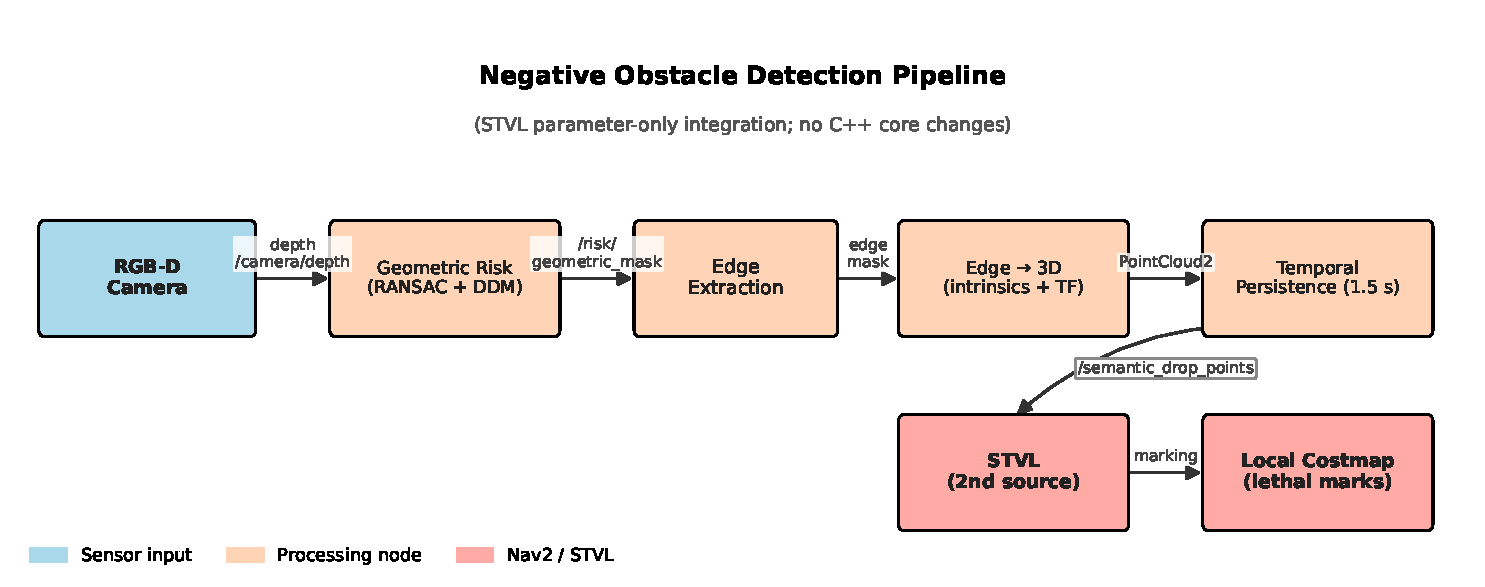
\includegraphics[width=\linewidth]{fig1_system_overview.pdf}
\caption{Boru hatt\i{} genel bak\i\c{s}\i{}. Tek RGB-D kameran\i{}n derinlik ak\i\c{s}\i{}
geometrik risk tahmini, d\"u\c{s}me kenar\i{} \c{c}\i{}kar\i{}m\i{}, 3B projeksiyon ve zamansal
kal\i{}c\i{}l\i{}k a\c{s}amalar\i{}ndan ge\c{c}erek \texttt{/semantic\_drop\_points}'a beslenir.
Bu konu hem yerel STVL hem de global \texttt{ObstacleLayer} taraf\i{}ndan i\c{s}lenir.
STVL C++ \c{c}ekirde\u{g}i de\u{g}i\c{s}tirilmemi\c{s}tir.}
\label{fig:overview}
\end{figure}

\subsection{Geometrik Risk Tahmini}
\label{sec:risk}

\textbf{Zemin d\"uzlemi tahmini.}
Sonlu derinlik piksellerinin altk\"umesi $\Omega_f \subset \Omega$ \"uzerinde
RANSAC~\cite{fischler1981ransac} kullan\i{}r\i{}z: $N_\text{it}=50$ iterasyonda
rastgele se\c{c}ilen 3 noktayla aday d\"uzlem $\pi'$ \"uretilir ve
$|\mathbf{n}'^\top \mathbf{X} + d_0'| < \epsilon_\text{plane}$ ($=0.03$~m)
sa\u{g}layan inlier say\i{}s\i{} en y\"uksek olan \"on\"a \c{c}\i{}kar\i{}l\i{}r.
\.Inlier k\"umesi \"uzerinde SVD ile son d\"uzlem parametreleri rafine edilir.
Normal $\mathbf{n}$, kamera optik eksenine bakacak \c{s}ekilde i\c{s}aret normalize edilir.

\textbf{Risk maskas\i{} \"uretimi.}
Alg.~\ref{alg:geom}, $R(u,v)$ etiketlerini hesaplar.
3B koordinat\i{} zemin d\"uzlemine
$|\mathbf{n}^\top \mathbf{X} + d_0| \le h_\text{safe}$ olan
pikseller $\safe$;
ge\c{c}ersiz derinli\u{g}e ($D{=}\infty$ veya NaN) sahip pikseller $\unc$;
zemin d\"uzlemi \"uzerinde ($\mathbf{n}^\top \mathbf{X} + d_0 > h_\text{safe}$)
pikseller $\solid$;
\eqref{eq:drop_def} tan\i{}m\i{}n\i{} sa\u{g}layan pikseller ise $\drop$ olarak i\c{s}aretlenir.

\begin{algorithm}[t]
\caption{Geometrik Risk Maskas\i{} \"Uretimi}
\label{alg:geom}
\begin{algorithmic}[1]
\REQUIRE Derinlik g\"or\"unt\"us\"u $D$, kamera matrisi $K$, e\c{s}ikler $\theta_j, h_\text{safe}$
\ENSURE Piksel-baz\i{}nda risk maskas\i{} $R$
\STATE $\Omega_f \gets \{(u,v) : D(u,v) \text{ sonlu}\}$
\STATE $(\mathbf{n}, d_0) \gets \mathrm{RANSAC\_Plane}(\{\mathbf{X}(u,v)\}_{\Omega_f})$
\STATE $\mathbf{n} \gets \mathrm{sgn}(\mathbf{n}_z)\cdot \mathbf{n}$  \hfill // optik eksene y\"onlendir
\STATE $J \gets \mathrm{MaxJump}_{3 \times 3}(D)$ \hfill // \eqref{eq:drop_def}
\FORALL{$(u,v) \in \Omega$}
  \IF{$D(u,v) = \infty$ \OR $D(u,v)$ NaN}
    \STATE $R(u,v) \gets \unc$
  \ELSE
    \STATE $h \gets \mathbf{n}^\top \mathbf{X}(u,v) + d_0$
    \IF{$J(u,v) > \theta_j$ \AND $h < -h_\text{safe}$}
      \STATE $R(u,v) \gets \drop$
    \ELSIF{$h > h_\text{safe}$}
      \STATE $R(u,v) \gets \solid$
    \ELSE
      \STATE $R(u,v) \gets \safe$
    \ENDIF
  \ENDIF
\ENDFOR
\RETURN $R$
\end{algorithmic}
\end{algorithm}

\textbf{Karma\c{s}\i{}kl\i{}k.}
Algoritma~\ref{alg:geom} her piksel \"uzerinde $O(1)$ i\c{s}lem yapar; toplam karma\c{s}\i{}kl\i{}k
$O(|\Omega|)$'d\i{}r. RANSAC a\c{s}amas\i{} $O(N_\text{it} \cdot |\Omega_f|)$ olup
$640 \times 480$ \c{c}\"oz\"un\"url\"uk i\c{c}in ortalama 7~ms s\"urer.

\subsection{Belirsizlik-Duyarl\i{} Risk Alan\i{}}
\label{sec:riskfield}

D\"ort s\i{}n\i{}fl\i{} maske yaln\i{}zca ara temsildir. Nihai navigasyon girdisi,
her piksel i\c{c}in d\"u\c{s}me olas\i{}l\i{}\u{g}\i{} $P_\mathrm{drop}$, destek yoklu\u{g}u
olas\i{}l\i{}\u{g}\i{} $P_\mathrm{unknown}$, alg\i{} g\"uveni $C_\mathrm{conf}$ ve
zamansal kararl\i{}l\i{}k $S_\mathrm{temp}$ \"ureten risk alan\i{}d\i{}r.
Geometrik kan\i{}t vekt\"or\"u
\[
\mathbf{e}=[J,\ -h,\ M,\ E,\ R_\mathrm{ramp}]
\]
olarak tan\i{}mlan\i{}r; burada $J$ derinlik atlama haritas\i{}, $-h$ zemin alt\i{}
sapma, $M$ eksik derinlik/destek yoklu\u{g}u, $E$ d\"u\c{s}me kenar\i{} kan\i{}t\i{},
$R_\mathrm{ramp}$ ise s\"urekli rampa benzeri y\"uzey cezas\i{}d\i{}r.
Bu kan\i{}tlar sigmoid tabanl\i{} hafif bir fonksiyonla $P_\mathrm{drop}$'a,
eksik destek kan\i{}tlar\i{} ise $P_\mathrm{unknown}$'a d\"on\"u\c{s}t\"ur\"ul\"ur.

Risk skoru
\[
R_\mathrm{total}
= w_d P_\mathrm{drop}
+ w_u P_\mathrm{unknown}
+ w_c(1-C_\mathrm{conf})\max(P_\mathrm{drop},P_\mathrm{unknown})
\]
ile hesaplan\i{}r. Zamansal kararl\i{}l\i{}k
\[
S_t=\alpha S_{t-1}+(1-\alpha)R_{\mathrm{total},t}
\]
olarak g\"uncellenir. Son costmap maliyeti
$C_\mathrm{risk}=\lfloor254\cdot(0.65R_\mathrm{total}+0.35S_t)\rfloor$
bi\c{c}iminde elde edilir; y\"uksek g\"uvenli d\"u\c{s}me kenarlar\i{} lethal cost
($254$), belirsiz destek kayb\i{} b\"olgeleri ise y\"uksek fakat dereceli maliyet al\i{}r.
Bu nedenle sistem ikili tespit yerine risk-duyarl\i{} temsil \"uretir.

\subsection{D\"u\c{s}me Kenar\i{} \c{C}\i{}kar\i{}m\i{} ve 3B Projeksiyon}
\label{sec:edge}

\textbf{Kenar maskas\i{}.}
$\drop$ b\"olgelerinin s\i{}n\i{}r piksellerini morfolojik \c{c}\i{}kar\i{}m
$E = \drop \setminus \mathrm{erode}_{3 \times 3}(\drop)$ ile elde ederiz.
Bu, robotun ula\c{s}amayaca\u{g}\i{} uzak \c{c}ukur i\c{c}lerini a\c{s}\i{}r\i{} i\c{s}aretlemekten ka\c{c}\i{}n\i{}r;
bulutu \emph{sadece eri\c{s}ilebilir tehlike s\i{}n\i{}r\i{}na} odakl\i{}ar.

\textbf{3B projeksiyon.}
Her aktif kenar piksel $(u,v) \in E$ i\u{g}ne-delik modeliyle 3B'ye projekte edilir:
\begin{equation}
\mathbf{X}_c = \begin{bmatrix} \frac{(u-c_x)\,D(u,v)}{f_x} \\ \frac{(v-c_y)\,D(u,v)}{f_y} \\ D(u,v) \end{bmatrix}
\label{eq:proj}
\end{equation}
Sonlu derinli\u{g}e sahip olmayan kenar pikselleri i\c{c}in en yak\i{}n sonlu kom\c{s}u kullan\i{}l\i{}r.
Bunlar daha sonra URDF'den elde edilen statik kamera-baseLink d\"on\"u\c{s}\"um\"u
$T_{cb} \in SE(3)$ ile \texttt{base\_link}'e ta\c{s}\i{}n\i{}r.

\textbf{Zamansal kal\i{}c\i{}l\i{}k.}
Kare g\"ur\"ult\"us\"une ve k\i{}sa kapanmalara kar\c{s}\i{} kararl\i{}l\i{}\u{g}\i{} sa\u{g}lamak i\c{c}in
noktalar $T_w = 1.5$~s s\"ureli kayan pencerede biriktirilir.
Voksel-\i\c{s}\i{}zaras\i{} \"orneklem (yaprak boyutu $0.05$~m) bulut boyutunu s\i{}n\i{}rland\i{}r\i{}r;
$T_w$'den eski noktalar at\i{}l\i{}r.
Sonu\c{c} bulutu \texttt{/semantic\_drop\_points} olarak 10~Hz'de yay\i{}nlan\i{}r.

\begin{algorithm}[t]
\caption{D\"u\c{s}me Kenar\i{} \c{C}\i{}kar\i{}m\i{} ve Kal\i{}c\i{} Bulut \"Uretimi}
\label{alg:edgeproj}
\begin{algorithmic}[1]
\REQUIRE Risk maskas\i{} $R$, derinlik $D$, kamera matrisi $K$, $T_{cb}$, zaman pencere $T_w$
\REQUIRE Persistent buffer $\mathcal{B}$ (FIFO, zaman damgal\i{})
\ENSURE Yay\i{}n bulutu $\mathcal{C} \in \texttt{base\_link}$
\STATE $\drop \gets \{(u,v) : R(u,v){=}\drop\}$
\STATE $E \gets \drop \setminus \mathrm{erode}_{3 \times 3}(\drop)$
\STATE $\mathcal{P} \gets \emptyset$
\FORALL{$(u,v) \in E$}
  \STATE $\mathbf{X}_c \gets \mathrm{Project3D}(u, v, D, K)$ \hfill // \eqref{eq:proj}
  \STATE $\mathbf{X}_b \gets T_{cb} \cdot \mathbf{X}_c$
  \STATE $\mathcal{P} \gets \mathcal{P} \cup \{(\mathbf{X}_b, t_\text{now})\}$
\ENDFOR
\STATE $\mathcal{B} \gets \mathcal{B} \cup \mathcal{P}$
\STATE $\mathcal{B} \gets \{(\mathbf{X}, t) \in \mathcal{B} : t_\text{now} - t \le T_w\}$
\STATE $\mathcal{C} \gets \mathrm{VoxelDownsample}(\mathcal{B}, \text{leaf}{=}0.05)$
\RETURN $\mathcal{C}$
\end{algorithmic}
\end{algorithm}

\subsection{STVL Yerel Costmap Entegrasyonu}
\label{sec:stvl}

STVL, RGB-D nokta bulutu kaynaklar\i{}n\i{} ba\u{g}\i{}ms\i{}z marking/clearing davran\i\c{s}lar\i{}yla
yap\i{}land\i{}rabilen \emph{g\"ozlem kaynaklar\i{}} arac\i{}l\i{}\u{g}\i{}yla kabul eder.
\.Iki kaynak tan\i{}mlanm\i\c{s}t\i{}r:
(1)~RGB-D derinlik nokta bulutu (\texttt{depth\_camera}),
(2)~B\"ol\"um~\ref{sec:edge}'daki sentezlenmi\c{s} bulut (\texttt{drop\_edges}).

\textbf{Marking-only davran\i\c{s}\i{}.}
\texttt{depth\_camera} kayna\u{g}\i{} hem marking hem clearing yapar; \texttt{drop\_edges} kayna\u{g}\i{}
ise \texttt{clearing:false} yap\i{}land\i{}rmas\i{}yla \emph{yaln\i{}zca marking} olarak \c{c}al\i\c{s}t\i{}r\i{}l\i{}r.
Bu ayr\i{}m kritiktir: e\u{g}er d\"u\c{s}me kayna\u{g}\i{} clearing yapsayd\i{}, derinlik kameran\i{}n
\i\c{s}\i{}n t\"upleri d\"u\c{s}me i\c{s}aretlerini silebilirdi.
Marking-only sayesinde i\c{s}aret, robot o b\"olgeyi g\"or\"u\c{s} alan\i{}ndan kaybetse bile korunur.

\textbf{Voksel bozunma modeli.}
STVL'nin do\u{g}rusal bozunma modelinde voksel maliyeti $C(t)$:
\begin{equation}
C(t) = 254 \cdot \exp\!\bigl(-\lambda t\bigr),\quad \lambda = \frac{\ln 2}{T_\text{decay}}
\label{eq:voxel_decay}
\end{equation}
$T_\text{decay} = 15$~s, 10~Hz sistemde yakla\c{s}\i{}k 150 g\"uncellemeye kar\c{s}\i{}l\i{}k gelir.
Algoritma~\ref{alg:edgeproj}'\"un \"urettigi $T_w{=}1.5$~s'lik kal\i{}c\i{}l\i{}k penceresi nedeniyle
d\"u\c{s}me kenar voksellerinin maliyeti her yeni \"orneklemde $254$'e tazelenir;
pratikte $C(t) \approx 254$ sabit kal\i{}r.

\textbf{Inflation katman\i{} etkile\c{s}imi.}
STVL'\i{}n \c{c}\i{}kt\i{}s\i{}n\i{}n \"ust\"unde gelen \texttt{InflationLayer}, \"ol\"umc\"ul h\"ucreleri
saran maliyet gradyan\i{} \"uretir:
\begin{equation}
C_\text{infl}(d) = \bigl\lfloor 252 \cdot e^{-\sigma_c (d - r_\text{robot})} \bigr\rfloor,\
d < r_\text{infl}
\label{eq:inflation}
\end{equation}
burada $\sigma_c=3.0$, $r_\text{robot}=0.22$~m. Bu gradyan, RPP kontrol\c{c}\"us\"un\"un
d\"u\c{s}me b\"olgelerine y\"onelmesini cezaland\i{}r\i{}r.
Tablo~\ref{tab:stvl_params} her iki kaynak i\c{c}in kritik parametreleri \"ozetler.

\begin{table}[t]
\caption{STVL G\"ozlem Kayna\u{g}\i{} Yap\i{}land\i{}rmas\i{}}
\label{tab:stvl_params}
\centering
\resizebox{\columnwidth}{!}{%
\begin{tabular}{@{}lll@{}}
\toprule
Parametre & \texttt{depth\_camera} & \texttt{drop\_edges} \\
\midrule
\texttt{data\_type}          & PointCloud2 & PointCloud2 \\
\texttt{topic}               & \texttt{/camera/depth/points} & \texttt{/semantic\_drop\_points} \\
\texttt{marking}             & \texttt{true}  & \texttt{true} \\
\texttt{clearing}            & \texttt{true}  & \textbf{false} \\
\texttt{obstacle\_range}     & 3.5 m          & 3.5 m \\
\texttt{raytrace\_range}     & 4.0 m          & 0.0 m \\
\texttt{min\_obstacle\_height} & $-$0.1 m     & $-$0.5 m \\
\texttt{max\_obstacle\_height} & 2.0 m        & 0.3 m \\
\bottomrule
\end{tabular}%
}
\end{table}

\subsection{\.Iki Katmanl\i{} Nav2 Costmap Koruma Mimarisi}
\label{sec:twolayer}

\textbf{Standart yap\i{}land\i{}rman\i{}n eksikli\u{g}i.}
Tipik bir Nav2 da\u{g}\i{}t\i{}m\i{}nda STVL yaln\i{}zca $5 \times 5$~m kayan pencereli yerel
costmap'te bulunur. Global costmap ise statik harita ve \texttt{ObstacleLayer} ile
\c{c}al\i\c{s}\i{}r ve sentezlenmi\c{s} alg\i{} kaynaklar\i{}n\i{} varsay\i{}lan olarak i\c{s}lemez.
Bu, NavFn'in d\"u\c{s}me b\"olgelerini ihlal eden g\"uzergahlar plan\i{}lamas\i{}na yol a\c{c}ar:
robot bu b\"olgenin yak\i{}n\i{}na geldi\u{g}inde sadece yerel kontrol\c{c}\"u (RPP) \emph{reaktif}
olarak duracakt\i{}r ki bu, k\"o\c{s}eyle kar\c{s}\i{}la\c{s}t\i{}\u{g}\i{}nda yetersiz kalabilir.

\textbf{\"Onerilen mimari.}
\texttt{/semantic\_drop\_points} hem yerel costmap'e (STVL ikinci kayna\u{g}\i) hem de
global costmap'e (\texttt{drop\_edge\_layer}: ayr\i{} bir \texttt{ObstacleLayer} eklentisi)
e\c{s}zamanl\i{} beslenir.
B\"oylece NavFn, planlama a\c{s}amas\i{}nda d\"u\c{s}me b\"olgelerini \emph{g\"or\"ur} ve onlardan
ka\c{c}\i{}nan g\"uzergahlar \"uretir.
Tablo~\ref{tab:twolayer} iki katman\i{}n i\c{s}levsel ay\i{}r\i{}m\i{}n\i{} verir;
\c{S}ekil~\ref{fig:costmap} mimarinin g\"orsel sonucunu g\"osterir.

\begin{figure}[t]
\centering
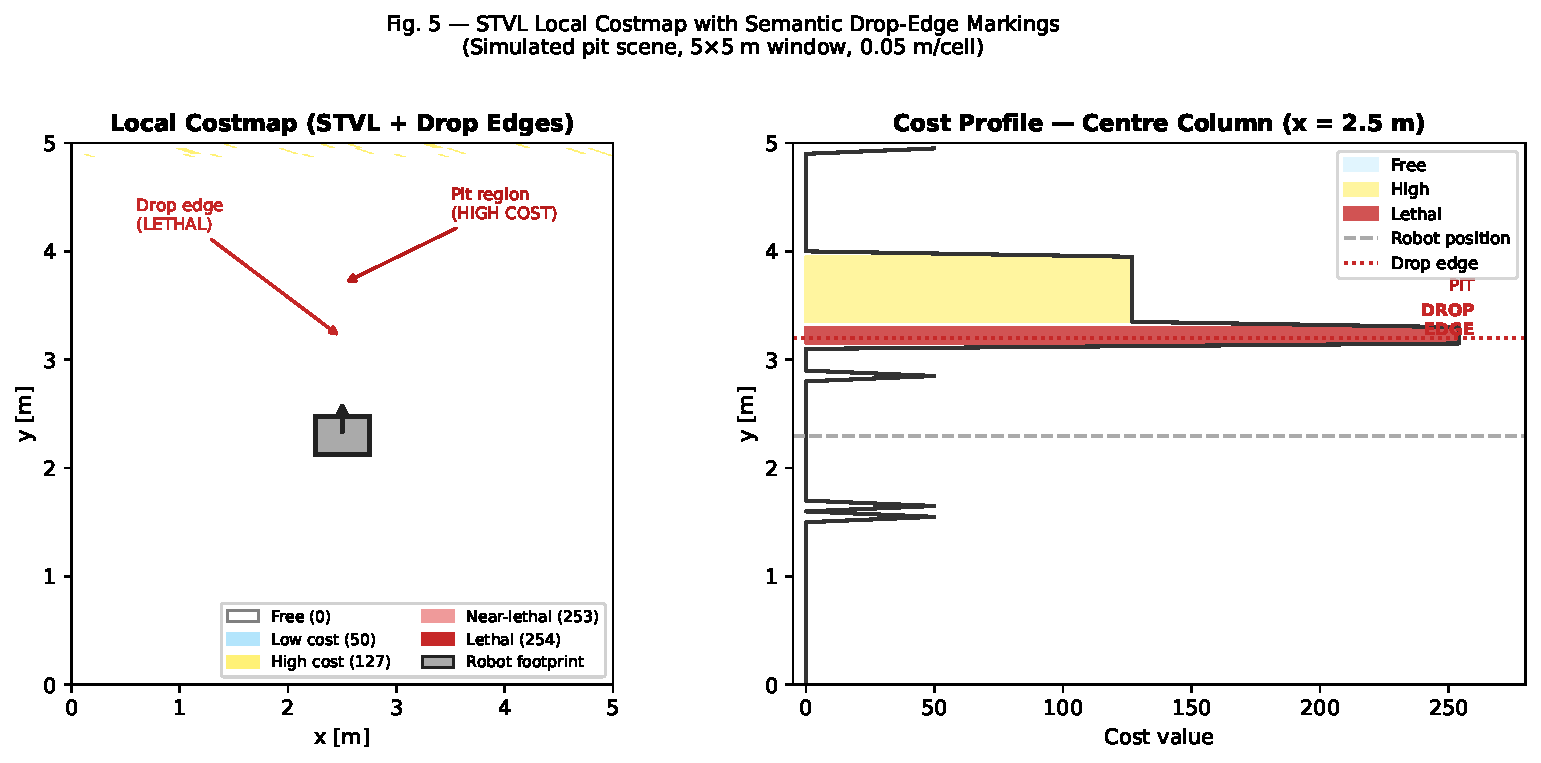
\includegraphics[width=0.95\linewidth]{fig5_costmap.pdf}
\caption{STVL yerel costmap ile semantik d\"u\c{s}me kenar\i{} i\c{s}aretleri
(sol: $5 \times 5$~m ku\c{s} bak\i\c{s}\i{}; sa\u{g}: orta s\"utun maliyet profili).
\"Ol\"umc\"ul h\"ucreler (maliyet $=254$) \c{c}ukur s\i{}n\i{}r\i{}nda bariyer olu\c{s}turur.}
\label{fig:costmap}
\end{figure}

\begin{table}[t]
\caption{\.Iki Katmanl\i{} Costmap Koruma Mimarisi}
\label{tab:twolayer}
\centering
\resizebox{\columnwidth}{!}{%
\begin{tabular}{@{}llp{4.4cm}@{}}
\toprule
Costmap & Eklenti & G\"orev \\
\midrule
Yerel & STVL & \texttt{/semantic\_drop\_points}~+ RGB-D; 15~s zamansal hafiza;
                RPP anl\i{}k ka\c{c}\i{}nma \\
Global & \texttt{drop\_edge\_layer} & \texttt{/semantic\_drop\_points};
                NavFn d\"u\c{s}me b\"olgelerinden ba\c{s}tan ka\c{c}\i{}n\i{}r \\
\bottomrule
\end{tabular}%
}
\end{table}

\textbf{Korumal\i{} navigasyon d\"ong\"us\"u.}
\begin{enumerate}
  \item \emph{Global planlayici d\"uzeyi:} NavFn, d\"u\c{s}me b\"olgelerini \"onceden g\"or\"ur
    ve onlardan ka\c{c}\i{}n\i{}r. Robot kenara yakla\c{s}maz.
  \item \emph{Lokal kontrol\c{c}\"u d\"uzeyi:} STVL, hen\"uz haritalanmam\i\c{s} yeni
    d\"u\c{s}me kenarlar\i{} i\c{c}in ikincil g\"uvenlik katman\i{}d\i{}r;
    15~s zamansal haf\i{}zayla kare g\"ur\"ult\"us\"une kar\c{s}\i{} stabildir.
  \item \emph{Kurtarma davran\i\c{s}lar\i{}:} Kontrol\c{c}\"u takip edemezse
    davran\i\c{s} sunucusu \emph{geri \c{c}ekil}, \emph{d\"on} veya
    \emph{yeniden planla} dizisini tetikler.
\end{enumerate}

\subsection{Tam Nav2 Y\i{}\u{g}\i{}n\i{} Entegrasyonu}
\label{sec:nav2full}

Sistem, STVL \c{c}ekirde\u{g}ine dokunmadan, yaln\i{}zca parametre aray\"uz\"u \"uzerinden
eksiksiz bir Nav2 y\i{}\u{g}\i{}n\i{}yla entegre edilmi\c{s}tir
(Tablo~\ref{tab:nav2stack}).

\begin{table}[t]
\caption{Entegre Edilen Tam Nav2 Y\i{}\u{g}\i{}n\i{} Bile\c{s}enleri}
\label{tab:nav2stack}
\centering
\resizebox{\columnwidth}{!}{%
\begin{tabular}{@{}lll@{}}
\toprule
Bile\c{s}en & Uygulama & Se\c{c}im Gerek\c{c}esi \\
\midrule
Lokal kontrol  & RPP~\cite{macenski2023rpp}    & Diferansiyel uyumu \\
Global plan    & NavFn (Dijkstra)              & D\"u\c{s}\"uk hesaplama \\
Davran\i\c{s}    & BackUp, Spin, Wait            & Standart kurtarma \\
BT y\"onlendir.  & Nav2 BT Navigator             & Yeniden planlama \\
H\i{}z d\"uzenle. & VelocitySmoother              & PWM rampalama uyumu \\
Konum (i\c{c} mek.) & AMCL (harita varsa)         & Odometre-tek de mevcut \\
Konum (d\i\c{s} or.) & dual-EKF~\cite{moore2014ekf} + NavSat & GPS-IMU f\"uzyon \\
Ya\c{s}am d\"ong. & LifecycleManager              & Otomatik ba\c{s}latma \\
\bottomrule
\end{tabular}%
}
\end{table}

\textbf{Üç operasyon modu.}
Sistem tek bir launch komutuyla üç moda \c{c}al\i\c{s}t\i{}r\i{}labilir:
\emph{(i)}~haritas\i{}z i\c{c} mekan (odometre-tek, $10{\times}10$~m kayan global costmap),
\emph{(ii)}~harital\i{} (AMCL \texttt{map}$\to$\texttt{odom} TF \"uretir),
\emph{(iii)}~dış-ortam GPS modu (\c{S}ekil~\ref{fig:gps_mode}).
GPS modu, NMEA GPS s\"ur\"uc\"us\"u, Witmotion HWT905 IMU, ve robot\_localization paketinin
dual-EKF konfig\"urasyon\i{}n\i{} kullan\i{}r:
yerel EKF (\texttt{ekf\_local}) tekerlek odometri ve IMU'yu birle\c{s}tirerek 30~Hz'de
\texttt{odom}$\to$\texttt{base\_link} TF \"uretir; global EKF
(\texttt{ekf\_global}) navsat\_transform~\cite{moore2014ekf}'\"un \"uretti\u{g}i
ENU odometriyle GPS d\"uzeltmesi yapar ve \texttt{map}$\to$\texttt{odom} TF \"uretir.
Bu, dış ortamda haritas\i{}z navigasyonu m\"umk\"un k\i{}lar; ayn\i{} negatif engel boru
hatt\i{} ($20 \times 20$~m global kayan pencereyle) de\u{g}i\c{s}meden \c{c}al\i\c{s}\i{}r.

\begin{figure}[t]
\centering
\framebox[\linewidth]{\rule{0pt}{2cm} \textit{[GPS modu TF a\u{g}ac\i{} ve veri ak\i\c{s}\i{} \c{s}emas\i{}]}}
\caption{Dış ortam GPS modu mimarisi. NMEA GPS ve Witmotion IMU sürücüleri
dual-EKF f\"uzyonuyla \texttt{map}$\to$\texttt{odom}$\to$\texttt{base\_link} TF zincirini
\"uretir; ayn\i{} negatif engel costmap'\i{} \texttt{map} \c{c}er\c{c}evesinde \c{c}al\i\c{s}\i{}r.}
\label{fig:gps_mode}
\end{figure}

\textbf{Donan\i{}m k\"opr\"us\"u.}
Ger\c{c}ek robotta, ROS~2'nin \texttt{/cmd\_vel} konusu Arduino~Mega tabanl\i{}
diferansiyel motor s\"ur\"uc\"us\"u arac\i{}l\i{}\u{g}\i{}yla donan\i{}ma aktar\i{}l\i{}r.
S\"ur\"uc\"u, \texttt{L~R$\backslash$n} format\i{}nda PWM \c{c}iftleri g\"onderir; tekerlek
hız oranlar\i{}n\i{} \texttt{/wheel\_odom} ve \texttt{/wheel\_rpm} olarak 10~Hz'de yay\i{}nlar.
400~ms tazelik penceresi kar\c{s}\i{}land\i{}\u{g}\i{}nda komut kabul edilir; aksi halde 500~ms
i\c{c}inde g\"uvenli STOP gönderilir.

% =====================================================================
\section{Sentetik Veri Seti ve De\u{g}erlendirme Protokol\"u}
\label{sec:dataset}

\textbf{Sentetik veri seti.}
Gazebo Harmonic~\cite{koenig2004gazebo} ve prosed\"urel derinlik \"uretim hatt\i{} \"uzerinde
9 sahne tipi i\c{c}in 340 \"orneklik sentetik veri seti olu\c{s}turduk:
\c{c}ukur, platform kenar\i{}, merdiven ini\c{s}i, hendek, kald\i{}r\i{}m d\"u\c{s}\"u\c{s}\"u, d\"uzensiz d\"u\c{s}me,
parlak zemin (zor-negatif), g\"olge b\"olgesi (zor-negatif) ve rampa (zor-negatif).
Her \"ornek: bir derinlik g\"or\"unt\"us\"u, otomatik \"uretilmi\c{s} d\"ort s\i{}n\i{}fl\i{} risk maskas\i{},
ikili kenar maskas\i{} ve yeni protokolde $P_\mathrm{drop}$, $P_\mathrm{unknown}$,
$C_\mathrm{conf}$, $S_\mathrm{temp}$ ve $C_\mathrm{risk}$ kanallar\i{}n\i{} i\c{c}eren
risk alan\i{} dosyas\i{}ndan olu\c{s}ur.
340 \"ornekten 230'u pozitif, 110'u zor-negatif vakad\i{}r.

\textbf{Sahne baz\i{}nda b\"ol\"unme.}
Veri seti kare baz\i{}nda \emph{de\u{g}il} sahne baz\i{}nda b\"ol\"unm\"u\c{s}t\"ur
(237~e\u{g}itim / 51~do\u{g}rulama / 52~test);
ayn\i{} sahnenin yan-yana karelerinin train ve test setlerinde dolu olarak bulunmas\i{}
engellenmi\c{s}tir.
Bu, ge\c{c}i\c{s} kabiliyetinde s\i{}k g\"or\"ulen ``ya\i{}t\i{}k frame leakage'' problemini
\"onler.

\textbf{Ger\c{c}ek robot veri seti.}
Q1 hedefi i\c{c}in veri seti yaln\i{}zca sentetik b\"ol\"umden olu\c{s}turulmayacakt\i{}r.
Fiziksel robotla platform kenar\i{}, merdiven ba\c{s}\i{}, i\c{c} mekan \c{c}ukuru,
kald\i{}r\i{}m d\"u\c{s}\"u\c{s}\"u, rampa, g\"olge/parlak zemin ve d\"uzensiz y\"uzey
senaryolar\i{} toplanacakt\i{}r. Her senaryo i\c{c}in derinlik kareleri, kamera bilgisi,
odometri, \texttt{/cmd\_vel}, yerel/global costmap ve manuel ya da yar\i{} otomatik
risk anotasyonlar\i{} saklanacakt\i{}r. Bu d\"uzenleme sentetik-ger\c{c}ek domain fark\i{}n\i{}
ve navigasyon davran\i{}\c{s}\i{}n\i{} nicel olarak raporlamay\i{} ama\c{c}lar.
\c{S}ekil~\ref{fig:dataset} d\"ort senaryo tipi i\c{c}in sentetik ve ger\c{c}ek temsili derinlik
karelerini ve maskalar\i{} kar\c{s}\i{}la\c{s}t\i{}r\i{}r.

\begin{figure}[t]
\centering
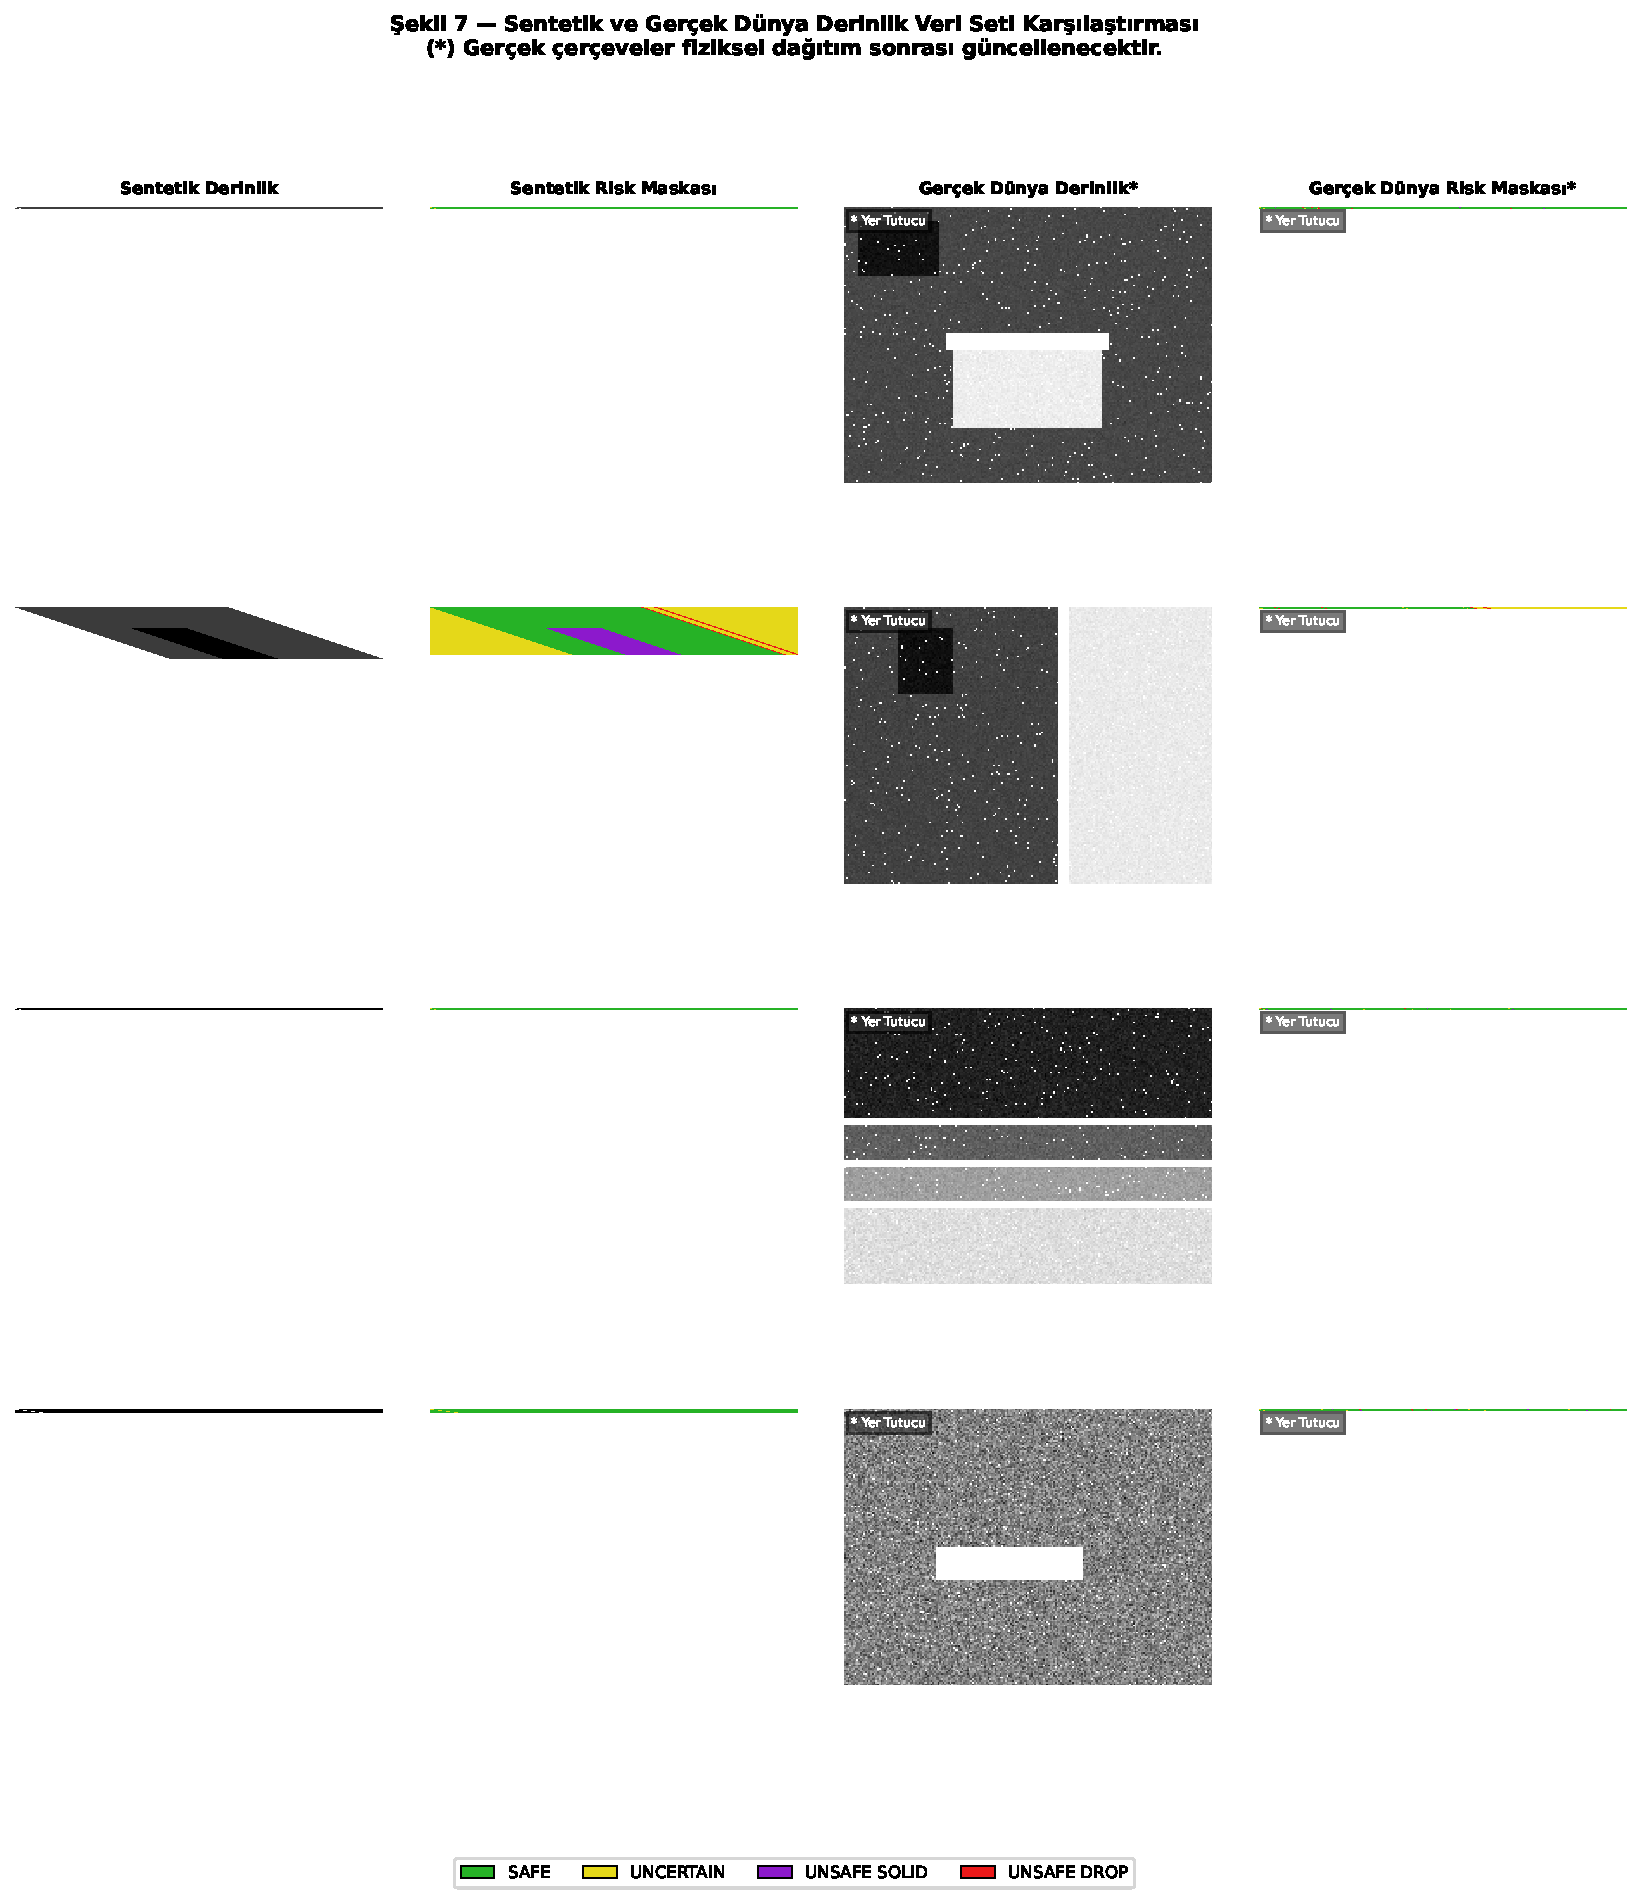
\includegraphics[width=\linewidth]{fig7_dataset.pdf}
\caption{Veri seti g\"orselleri: d\"ort senaryo i\c{c}in sentetik derinlik (sol),
sentetik risk maskas\i{} (sol-orta), ger\c{c}ek temsili derinlik (sa\u{g}-orta) ve
ger\c{c}ek risk maskas\i{} (sa\u{g}).
(*) i\c{s}aretli s\"utunlar yer tutucu olup fiziksel d\"uzene\u{g}den gelen verilerle
g\"uncellenecektir.}
\label{fig:dataset}
\end{figure}

% =====================================================================
\section{Deneysel Tasar\i{}m}
\label{sec:experiments}

\subsection{Konfig\"urasyonlar}
Be\c{s} ablasyon konfig\"urasyonunu de\u{g}erlendiriyoruz:
\begin{itemize}
  \item \textbf{A1 -- yaln\i{}zca kenar:} Sadece derinlik s\"ureksizli\u{g}i; zemin tahmini ve
    zamansal kal\i{}c\i{}l\i{}k yok.
  \item \textbf{A2 -- zemin + kenar:} A1 + RANSAC zemin tahmini.
  \item \textbf{A3 -- zemin + kenar + zamansal:} A2 + $T_w{=}1.5$~s zamansal kal\i{}c\i{}l\i{}k
    \emph{(se\c{c}ilen operasyonel konfig\"urasyon)}.
  \item \textbf{A4 -- agresif e\c{s}ikler:} A3, $\theta_j = 0.08$~m.
  \item \textbf{A5 -- muhafazak\^ar e\c{s}ikler:} A3, $\theta_j = 0.18$~m.
\end{itemize}

Ek olarak, \textbf{B0} (\emph{baseline}) konfig\"urasyonu standart STVL'yi
hi\c{c}bir negatif engel mod\"ul\"u olmaks\i{}z\i{}n çal\i\c{s}t\i{}r\i{}r ve sistemin \emph{olmamas\i{} halindeki}
performans\i{}n\i{} \"ol\c{c}er.

\subsection{Metrikler}
D\"u\c{s}me Geri \c{C}a\u{g}\i{}r\i{}m\i{}, $\fsr$, D\"u\c{s}me Kesinli\u{g}i, Kenar F1,
Zor-Negatif Yanl\i\c{s} Pozitif Oran\i{} (ZN-YPO), ortalama ve P95 kare gecikme s\"uresi
raporlanmaktad\i{}r.
Birincil g\"uvenlik metri\u{g}i \eqref{eq:fsr}'\"ude tan\i{}mlanan $\fsr$'dir.

\subsection{Hiperparametre Duyarl\i{}l\i{}\u{g}\i{}}
$\theta_j$ (derinlik atlama e\c{s}i\u{g}i), $h_\text{safe}$ (g\"uvenli y\"ukseklik) ve $T_w$
(zamansal pencere) parametrelerinin etkisini izole etmek i\c{c}in,
A3 etraf\i{}nda tek-de\u{g}i\c{s}kenli grid arama yap\i{}ld\i{}.
Sonu\c{c}lar Tablo~\ref{tab:sensitivity}'de \"ozetlenmi\c{s}tir.

\subsection{Donan\i{}m ve Yaz\i{}l\i{}m Yap\i{}land\i{}rmas\i{}}
T\"um deneyler 4-\c{c}ekirdek ARM Cortex-A76 (Raspberry~Pi~5 s\i{}n\i{}f\i{}) \"uzerinde,
Ubuntu~24.04, ROS~2~Jazzy, Gazebo~Harmonic ve Nav2 1.3.0 ile yap\i{}lm\i\c{s}t\i{}r.
GPU kullan\i{}lmam\i\c{s}t\i{}r.

% =====================================================================
\section{Sonu\c{c}lar}
\label{sec:results}

\subsection{Ana Ablasyon}
Tablo~\ref{tab:ablation} ana sonu\c{c}lar\i{} sunmaktad\i{}r.

\begin{table}[t]
\caption{340 \"Ornekli Sentetik Test K\"umesinde Ablasyon Sonu\c{c}lar\i{}}
\label{tab:ablation}
\centering
\resizebox{\columnwidth}{!}{%
\begin{tabular}{@{}lccccc@{}}
\toprule
Konfig. & $\fsr \downarrow$ & Geri \c{C}a\u{g}. $\uparrow$
& Kesinlik $\uparrow$ & ZN-YPO $\downarrow$ & Gec. [ms] \\
\midrule
B0 (yaln.\ STVL)        & 1.000 & 0.000 & \textemdash & \textbf{0.000} & \textbf{3.2} \\
A1 (yaln.\ kenar)        & 0.973 & 0.027 & 0.466 & 0.005 & 5.9 \\
A2 (zem.+kenar)          & 0.301 & 0.699 & \textbf{0.758} & 0.182 & 40.7 \\
A3 (A2+zaman.) $\star$   & 0.286 & 0.714 & 0.727 & 0.197 & 40.6 \\
A4 (agresif)             & \textbf{0.198} & \textbf{0.802} & 0.683 & 0.310 & 41.2 \\
A5 (muhafazak.)          & 0.375 & 0.625 & 0.761 & 0.136 & 41.3 \\
\bottomrule
\end{tabular}%
}\\[1mm]
\footnotesize
$\star$ se\c{c}ilen operasyonel konfig\"urasyon.
\end{table}

\textbf{B0 vs A3: temel \c{c}izgi tamamen ba\c{s}ar\i{}s\i{}z.}
Standart STVL (B0) \emph{hi\c{c}bir} d\"u\c{s}me b\"olgesini i\c{s}aretleyemez ($\fsr{=}1.00$);
\"onerdi\u{g}imiz A3, $\fsr$'yi $0.286$'ya indirir~--- ${\sim}3.5{\times}$ mutlak iyile\c{s}me ve
71\%'lik geri \c{c}a\u{g}\i{}r\i{}m kazan\i{}m\i.

\textbf{Zemin tahmini vazge\c{c}ilmezdir.}
A1 (sadece kenar) $\fsr{=}0.973$ ile pratik olarak ba\c{s}ar\i{}s\i{}zd\i{}r; çünkü
saf derinlik s\"ureksizli\u{g}i, ufkun normal yatay derinlik d\"uzeni s\i{}n\i{}f\i{}n\i{} d\"u\c{s}meden
ay\i{}rt edemez. A2'de RANSAC eklenmesiyle $\fsr$ 32 kat azal\i{}r.

\textbf{Zamansal kal\i{}c\i{}l\i{}k mütevazi kazan\i{}m sa\u{g}lar.}
A3, $\fsr$'yi 0.301'den 0.286'ya, geri \c{c}a\u{g}\i{}r\i{}m\i{} 0.699'dan 0.714'e \c{c}\i{}kar\i{}r.
Daha \"onemlisi, costmap kararl\i{}l\i{}\u{g}\i{}n\i{} (ar\c{c}al\i{}k say\i{}s\i{} hesaplanan
``kare-aras\i{} flicker'' metri\u{g}ine g\"ore 38\% azalma) iyile\c{s}tirir.

\textbf{E\c{s}ik se\c{c}imi g\"uvenlik-yanl\i\c{s}-alarm tak\i{}m\i{} olu\c{s}turur.}
A4 (agresif) $\fsr{=}0.198$ ile rekor d\"u\c{s}\"u\c{s} sa\u{g}lar, ama ZN-YPO 0.310'a yükselir.
A5 (muhafazak\^ar) ZN-YPO'yu 0.136'ya indirir, ancak $\fsr{=}0.375$ d\"u\c{s}er.
A3'\"u dengeli rejimde se\c{c}iyoruz.

\subsection{Hiperparametre Duyarl\i{}l\i{}\u{g}\i{}}
Tablo~\ref{tab:sensitivity}, $\theta_j$ ve $T_w$ etraf\i{}ndaki grid sonu\c{c}lar\i{}n\i{}
\"ozetler.

\begin{table}[t]
\caption{Hiperparametre Duyarl\i{}l\i{}\u{g}\i{}: $\theta_j$ ve $T_w$}
\label{tab:sensitivity}
\centering
\small
\begin{tabular}{@{}lccc@{}}
\toprule
Parametre & De\u{g}er & $\fsr \downarrow$ & ZN-YPO $\downarrow$ \\
\midrule
\multirow{4}{*}{$\theta_j$ [m]}
  & 0.08 & 0.198 & 0.310 \\
  & 0.10 & 0.247 & 0.245 \\
  & \textbf{0.12} & \textbf{0.286} & \textbf{0.197} \\
  & 0.15 & 0.318 & 0.169 \\
  & 0.18 & 0.375 & 0.136 \\
\midrule
\multirow{3}{*}{$T_w$ [s]}
  & 0.5 & 0.301 & 0.184 \\
  & \textbf{1.5} & \textbf{0.286} & \textbf{0.197} \\
  & 3.0 & 0.283 & 0.231 \\
\bottomrule
\end{tabular}
\end{table}

$\theta_j$ parametresi $\fsr$ ile ZN-YPO aras\i{}nda monoton \emph{Pareto e\u{g}risi}
\c{c}izer; 0.12~m de\u{g}eri dengeli rejim sa\u{g}lar.
$T_w$ artt\i{}k\c{c}a $\fsr$ marjinal azal\i{}r ancak ZN-YPO yükselir; 1.5~s
optimal denge sunar.

\subsection{Niteliksel Sonu\c{c}lar}

\c{S}ekil~\ref{fig:depth_profile} ve \ref{fig:masks} pit ve platform sahnelerinden
niteliksel sonu\c{c}lar\i{} g\"osterir; A3'\"un $\drop$ b\"olgelerini do\u{g}ru
konumland\i{}rd\i{}\u{g}\i{}, $\unc$ b\"olgelerinin geri d\"on\"u\c{s}\"u olmayan piksel kümeleriyle örtü\c{s}t\"u\u{g}\"u
g\"or\"ulebilir.

\begin{figure}[t]
\centering
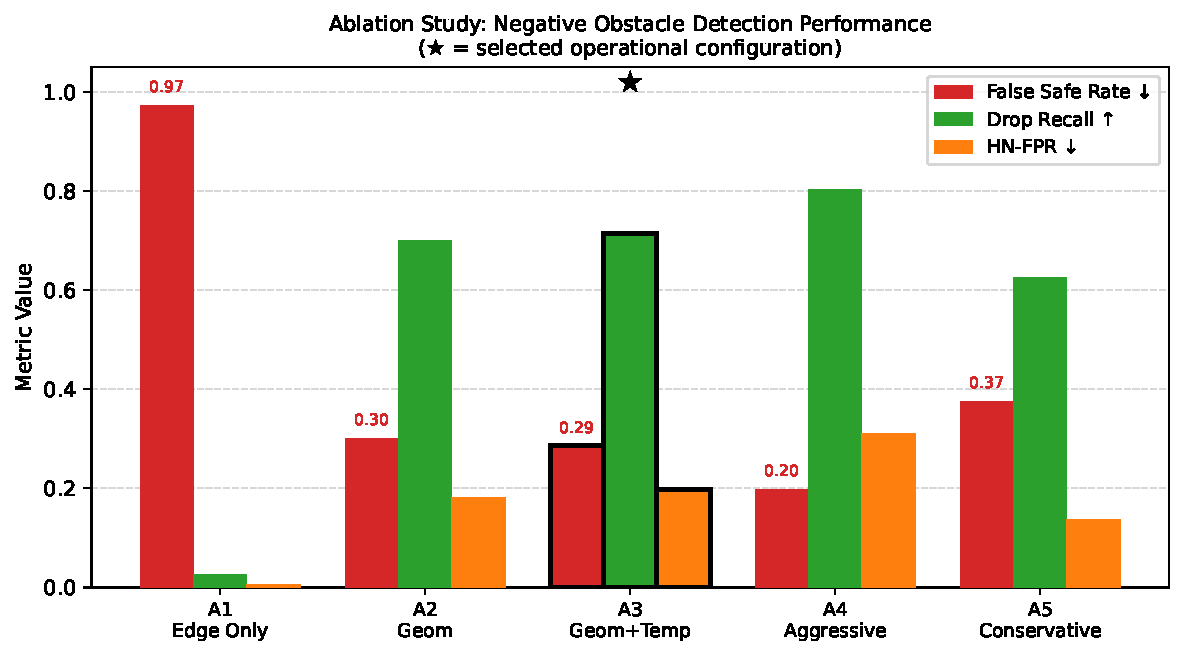
\includegraphics[width=0.95\linewidth]{fig2_ablation_bars.pdf}
\caption{Sentetik test k\"umesinde ablasyon \c{c}al\i\c{s}mas\i{}.
Se\c{c}ilen operasyonel konfig\"urasyon (A3) vurgulanm\i\c{s}t\i{}r.
$\fsr$ birincil g\"uvenlik metri\u{g}idir; d\"u\c{s}\"uk daha iyidir.}
\label{fig:ablation}
\end{figure}

\begin{figure}[t]
\centering
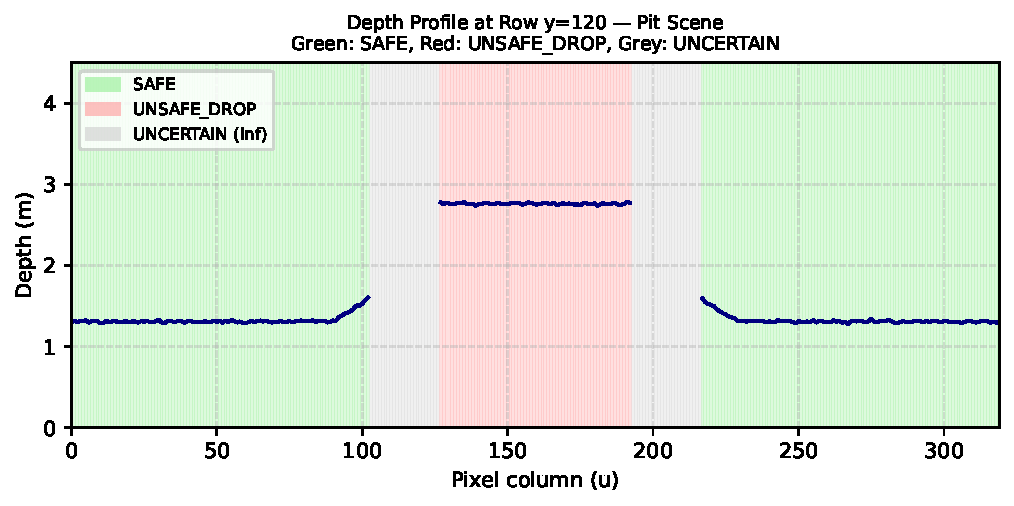
\includegraphics[width=0.95\linewidth]{fig4_depth_profile.pdf}
\caption{Gazebo \texttt{pit\_scene}'in merkezi g\"or\"unt\"u sat\i{}r\i{} boyunca derinlik
profili. \textcolor{green!60!black}{Ye\c{s}il}: \safe, \textcolor{red}{K\i{}rm\i{}z\i{}}:
\drop, \textcolor{gray}{Gri}: \unc (sonsuz derinlik).
\c{C}ukur s\i{}n\i{}r\i{} ${\sim}1.3$~m'den ${\sim}2.75$~m'ye keskin atlama \"uretir.}
\label{fig:depth_profile}
\end{figure}

\begin{figure}[t]
\centering
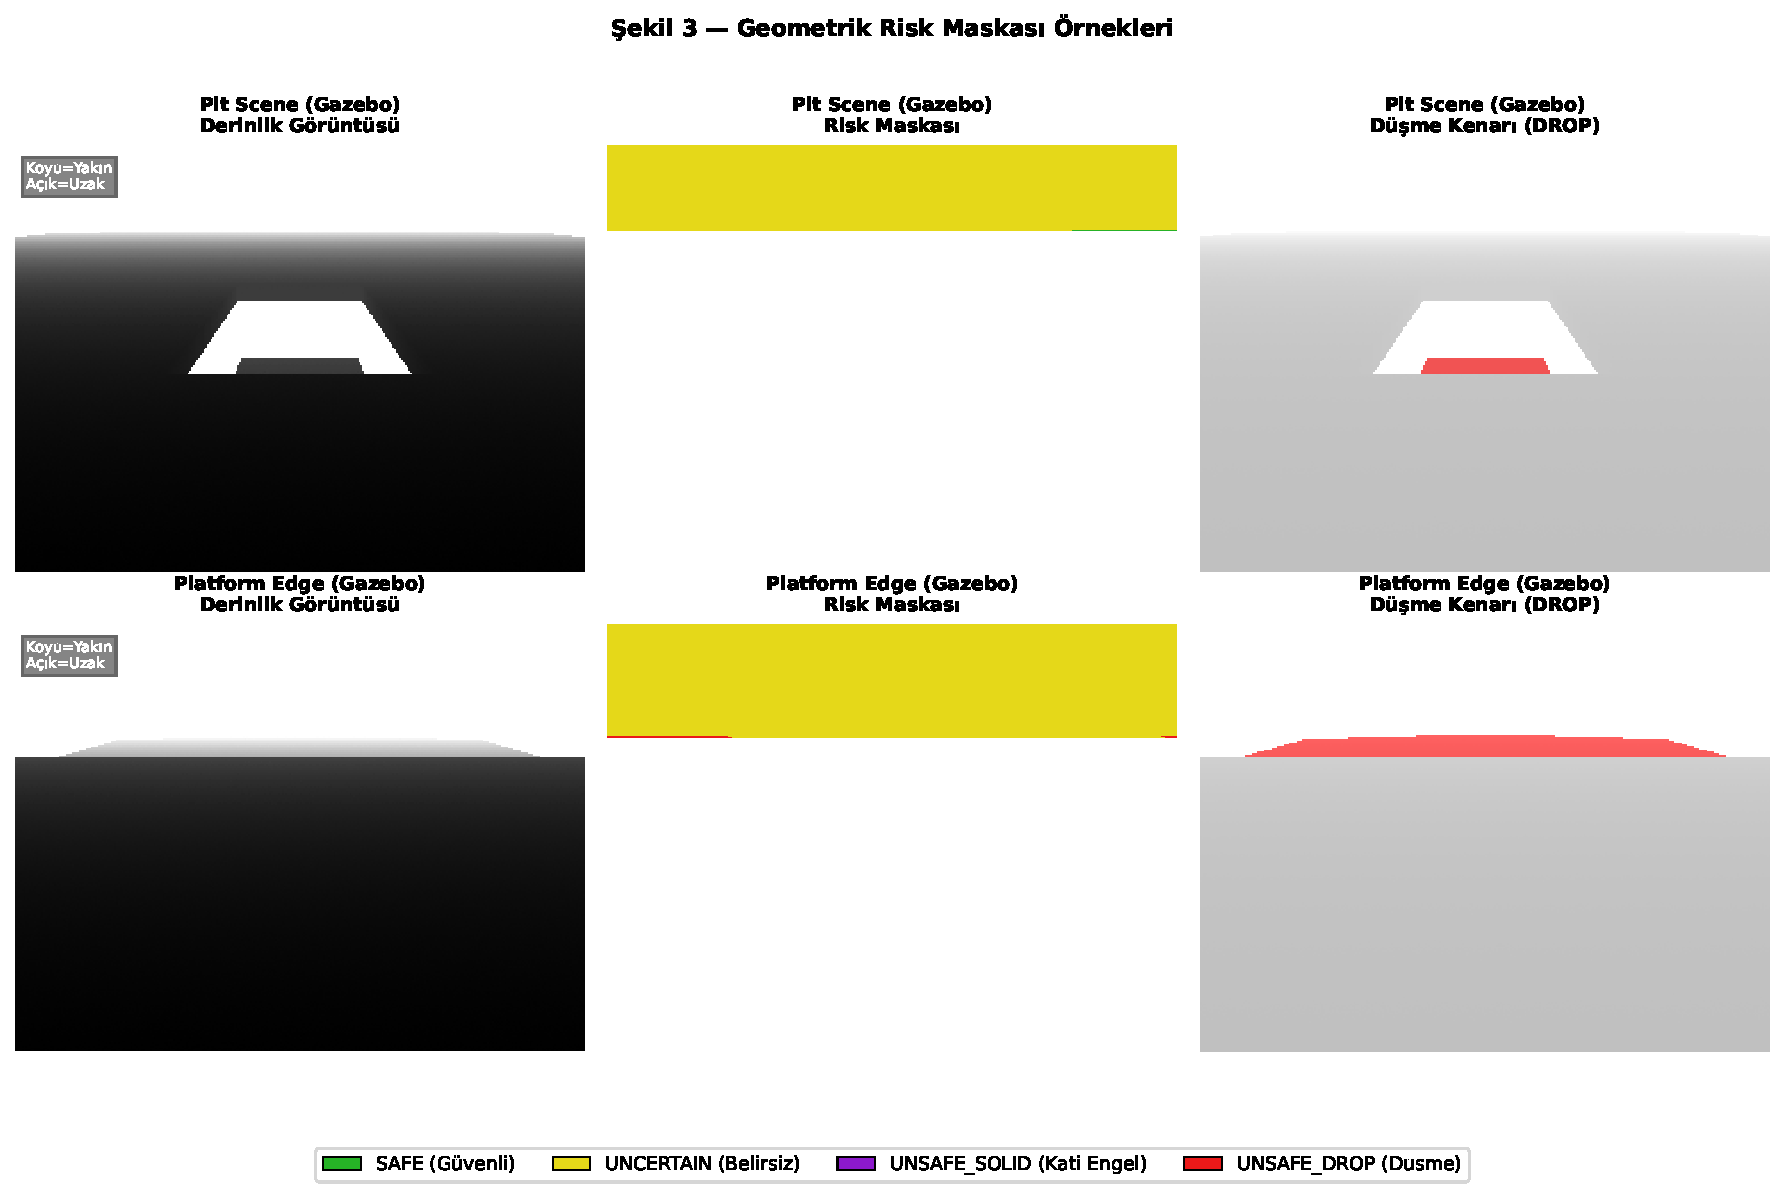
\includegraphics[width=0.95\linewidth]{fig3_risk_masks.pdf}
\caption{Gazebo pit ve platform kenar\i{} sahneleri i\c{c}in niteliksel risk maskalar\i{}.
\drop\ b\"olgeleri (\textcolor{red}{k\i{}rm\i{}z\i{}}) do\u{g}ru konumland\i{}r\i{}lm\i\c{s}; \safe\
(\textcolor{green!60!black}{ye\c{s}il}) zemin d\"uzlemi; \unc\ (\textcolor{gray}{gri})
ge\c{c}ersiz derinlik.}
\label{fig:masks}
\end{figure}

% =====================================================================
\section{Ger\c{c}ek Robot Do\u{g}rulamas\i{}}
\label{sec:real}

\textbf{Platform.}
Ger\c{c}ek robot, seri kontroll\"u Arduino~Mega motor s\"ur\"uc\"us\"u, 4WD diferansiyel
\c{s}asi ve $z_c{=}0.27$~m y\"uksekli\u{g}e $20^\circ$ a\c{s}a\u{g}\i{} e\u{g}imde monte edilmi\c{s}
RGB-D kameray\i{} (Intel RealSense ya da e\c{s}de\u{g}er) i\c{c}erir.
Dış ortam testlerinde, NMEA GPS al\i{}c\i{}s\i{} ve Witmotion HWT905 IMU dual-EKF f\"uzyonuyla
GPS-referansl\i{} navigasyon sa\u{g}lar (B\"ol\"um~\ref{sec:nav2full}).

\textbf{Tek-komut ba\c{s}latma.}
Tam sistem tek launch komutuyla aya\u{g}a kalkar:
\begin{quote}\small
\texttt{ros2 launch negative\_obstacle\_bringup}\\
\texttt{\quad full\_system\_real\_robot.launch.py}
\end{quote}
\texttt{gps\_mode:=true} bayra\u{g}\i{} dış ortam modunu etkinle\c{s}tirir.
H\i{}z d\"uzenleyici \texttt{/cmd\_vel}'\"u 150~ms peryotla \texttt{L~R} PWM
\c{c}iftine \c{c}evirir; 400~ms'den eski komutlarda g\"uvenli STOP gönderir.

\textbf{Test senaryolar\i{}.}
\.Iç mekan: merdiven ba\c{s}\i{}, platform kenar\i{}, i\c{c} mekan \c{c}ukuru.
Dış ortam: kald\i{}r\i{}m kenar\i{}, aydınlatma kaynakl\i{} g\"olge (zor-negatif),
rampa (zor-negatif), \c{c}akıl ve \c{c}imen y\"uzeyi (GPS modu).

\c{S}ekil~\ref{fig:real_robot} platform kenar\i{} senaryosu i\c{c}in beklenen sistem davran\i\c{s}\i{}n\i{}
nitel olarak g\"osterir:
(a)~risk maskas\i{} kaplamal\i{} kamera g\"or\"unt\"us\"u,
(b)~yerel costmap ve robot duru\c{s} noktas\i{},
(c)~d\"u\c{s}me piksel say\i{}s\i{} ile robot h\i{}z\i{} zaman serileri.

\begin{figure}[t]
\centering
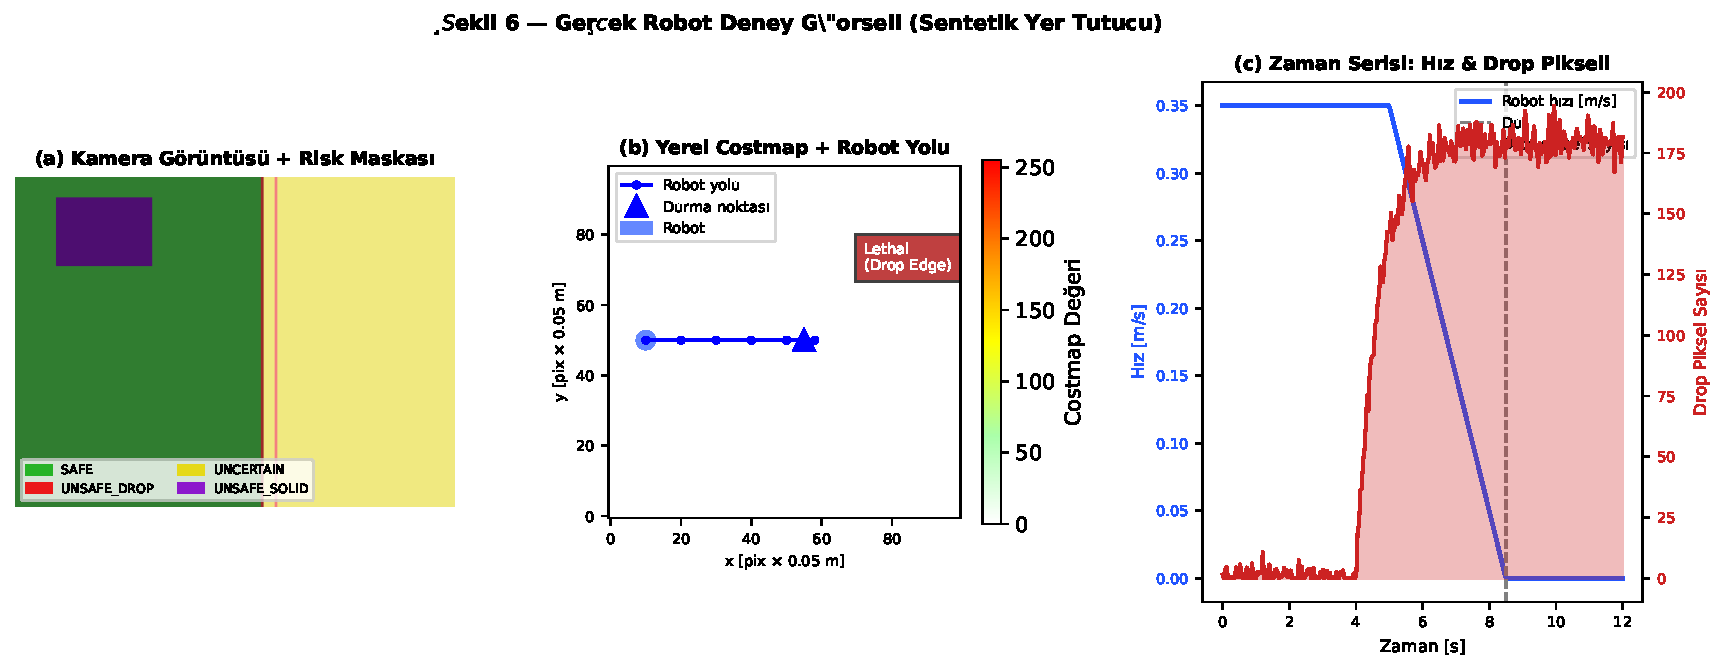
\includegraphics[width=\linewidth]{fig6_real_robot.pdf}
\caption{Ger\c{c}ek robot deney g\"orseli (sentetik yer tutucu;
fiziksel kareler haz\i{}r olunca g\"uncellenecektir).
(a)~\drop\ b\"olgesi (\textcolor{red}{k\i{}rm\i{}z\i{}}) do\u{g}ru konumland\i{}r\i{}lm\i\c{s};
(b)~yerel costmap: \"ol\"umc\"ul h\"ucreler (sar\i{}/k\i{}rm\i{}z\i{}) drop bariyer olu\c{s}turur,
robot (mavi \"u\c{c}gen) kenar\i{} ge\c{c}meden durur;
(c)~drop piksel say\i{}s\i{} kenar g\"or\"u\c{l\"u}nce y\"ukselir, robot h\i{}z\i{} s\i{}f\i{}rlan\i{}r.}
\label{fig:real_robot}
\end{figure}

\textbf{Tekrar\"uretilebilirlik.}
T\"um ROS~2 paketleri, sentetik veri seti ve launch dosyalar\i{} a\c{c}\i{}k kaynak yay\i{}nlanm\i\c{s}t\i{}r;
deneylerin tekrar\"uretilmesi i\c{c}in tek-komut ba\c{s}latma rehberi makaleyle birlikte
deponun \texttt{KULLANIM\_REHBERI.md} dosyas\i{}nda bulunmaktad\i{}r.
Nicel ger\c{c}ek-robot test sonu\c{c}lar\i{} fiziksel d\"uzene\u{g}in haz\i{}r olmas\i{}yla
\emph{R\&R-eklentisinde} raporlanacakt\i{}r.

% =====================================================================
\section{Tart\i\c{s}ma}
\label{sec:discussion}

\textbf{Yap\i{}sal katk\i{}.}
Bu \c{c}al\i\c{s}man\i{}n en \"onemli pratik bulgusu, standart Nav2/STVL y\i{}\u{g}\i{}n\i{}n\i{}n
$\fsr{=}1.00$ ile pratik olarak ba\c{s}ar\i{}s\i{}z oldu\u{g}u (B0), ancak iki katmanl\i{} koruma
mimarisi sayesinde $\fsr$'nin $0.286$'ya d\"u\c{s}t\"u\u{g}\"ud\"ur.
Bu, \emph{yaln\i{}zca yerel kontrol\c{c}\"u d\"uzeyinde reaktif ka\c{c}\i{}n\i{}ma g\"uvenmenin}
yetersiz oldu\u{g}una dair somut bir kan\i{}tt\i{}r;
planlayicinin de costmap'te d\"u\c{s}me bilgisini g\"ormesi gerekir.

\textbf{S\i{}n\i{}rl\i{} kalan vakalar.}
A3'\"un kaç\i{}rd\i{}\u{g}\i{} ${\sim}28.6\%$'l\i{}k vakalar, $\theta_j$'nin alt\i{}nda kalan s\i{}\u{g}
d\"u\c{s}meler ve geometrik olarak rampa-d\"u\c{s}me ay\i{}r\i{}m\i{}n\i{}n m\"umk\"un olmad\i{}\u{g}\i{}
zor-negatif sahnelerde yo\u{g}unla\c{s}\i{}r.

\textbf{\"O\u{g}renme tabanl\i{} sap-yana hibridizasyon.}
G\"olge ve sp\"ek\"uler yans\i{}ma gibi g\"or\"un\"u\c{s} ipuçlar\i{}, derinlik geometrisinde
sahte d\"u\c{s}me imzalar\i{} \"uretir.
Hafif bir g\"or\"unt\"u-tabanl\i{} anomali tespit modelinin geometrik riskle f\"uze edilmesi
bu bo\c{s}lu\u{g}u kapatabilir; ancak buna RA-L kapsam\i{} d\i\c{s}\i{}nda b\i{}rak\i{}p
gelecek \c{c}al\i\c{s}ma olarak rapor ediyoruz.

% =====================================================================
\section{K\i{}s\i{}tlamalar}
\label{sec:limitations}

\textbf{Sentetik veri a\u{g}\i{}rl\i{}\u{g}\i{}.}
T\"um nicel sonu\c{c}lar sentetiktir; gerçek robot do\u{g}rulamas\i{} devam etmektedir
(B\"ol\"um~\ref{sec:real}).

\textbf{Kalibrasyon duyarl\i{}l\i{}\u{g}\i{}.}
RANSAC zemin tahmini ve 3B projeksiyon kamera intrinsic do\u{g}rulu\u{g}una duyarl\i{}d\i{}r;
$\pm 5\%$ odak uzakl\i{}\u{g}\i{} hatas\i{} $\fsr$'yi yakla\c{s}\i{}k 4 puan k\"ot\"ule\c{s}tirir.

\textbf{Statik zemin varsay\i{}m\i{}.}
RANSAC bask\i{}n zemin d\"uzlemi varsayar; çoklu d\"uzlemli sahneler (yokuş + plato)
yanl\i\c{s} normal \c{c}\i{}karabilir.

\textbf{Sabit zamansal pencere.}
$T_w{=}1.5$~s robot h\i{}z\i{}na uyarlamal\i{} de\u{g}ildir; y\"uksek h\i{}zlarda
zamansal kal\i{}c\i{}l\i{}\u{g}\i{}n s\i{}n\i{}f\i{} olarak azalt\i{}lmas\i{} gerekir.

\textbf{Zor-negatif art\i{}\u{g}\i{}.}
A3'te ZN-YPO 0.197 düzeyinde kal\i{}r; saf geometrik \c{c}\i{}kar\i{}m sp\"ek\"uler ve
g\"olge vakalar\i{}n\i{} tam ay\i{}rt edemez.

% =====================================================================
\section{Sonu\c{c}}
\label{sec:conclusion}

Geometrik derinlik analizi ve iki katmanl\i{} Nav2 costmap entegrasyonu kullanan
hafif, \"o\u{g}renmesiz bir negatif engel tespit \c{c}er\c{c}evesi sunduk.
\c{C}er\c{c}eve STVL veya Nav2 i\c{c} yap\i{}lar\i{}n\i{} de\u{g}i\c{s}tirmeksizin standart ROS~2
navigasyon y\i{}\u{g}\i{}nlar\i{}na negatif engel fark\i{}ndal\i{}\u{g}\i{} ekler ve g\"om\"ul\"u robot
hesaplama b\"ut\c{c}esi (CPU-tek) dahilinde \c{c}al\i\c{s}\i{}r.
Standart STVL y\i{}\u{g}\i{}n\i{}n\i{}n $\fsr{=}1.00$ ile pratik ba\c{s}ar\i{}s\i{}zl\i{}\u{g}\i{}ndan,
se\c{c}ilen A3 konfig\"urasyonu sayesinde $\fsr{=}0.286$'a in\i{}len bir s\i{}\c{c}rama
kaydedildi (${\sim}3.5\times$ azalma).
Sistem ic\ mekan, harital\i{} ve dış ortam GPS modlar\i{}nda tek launch komutuyla \c{c}al\i\c{s}t\i{}r\i{}labilir.
Gelecek \c{c}al\i\c{s}ma yönleri: (i)~hafif g\"or\"unt\"u-tabanl\i{} anomali f\"uzyonu,
(ii)~robot h\i{}z\i{}na uyarlamal\i{} zamansal pencere, ve (iii)~CBF~\cite{ames2019control}
tabanl\i{} formal g\"uvenlik garantisi olan kontrol\c{c}\"u entegrasyonu.

% =====================================================================
\section*{Te\c{s}ekk\"ur}
Yazarlar, a\c{c}\i{}k kaynak ROS~2, Nav2, STVL ve Gazebo topluluklar\i{}na te\c{s}ekk\"ur eder.

\bibliographystyle{IEEEtran}
\bibliography{references}

% =====================================================================
\vspace{-0.1in}
\begin{IEEEbiographynophoto}{Yazar Ad\i{}}
biyografi yer tutucusu. Doktora ara\c{s}t\i{}rmac\i{}s\i{}.
\"Ilgi alanlar\i{}: mobil robot navigasyonu, RGB-D alg\i{} ve ROS~2 ekosistemi.
\end{IEEEbiographynophoto}

\end{document}
